%%%%%%%%%%%% Für Johannes %%%%%%%%%%%%
\newif\ifJCS
%\JCStrue
\ifJCS
	\documentclass[final,a4paper,DIV=calc,abstract,english]{scrartcl}
		\usepackage{setspace} % Change spacing
			%\singlespacing
			%\onehalfspacing
			\doublespacing
		\usepackage[none]{hyphenat}\raggedright % No hyphenation, but ugly output
		\setlength{\parindent}{10pt}
		\usepackage{endfloat}
		\usepackage{natbib}
\else
	\documentclass[a4paper,twocolumn=true,DIV=calc,abstract,english]{scrartcl}
		\usepackage[numbers,sort&compress]{natbib}
\fi
%%%%%%%%%%%% Für Johannes %%%%%%%%%%%%
\usepackage[utf8]{inputenc}
\usepackage{babel}
\usepackage[T1]{fontenc}
\usepackage{graphicx}
\usepackage{booktabs}
\usepackage{todonotes}
\usepackage[binary-units=true]{siunitx}
	\DeclareSIUnit\Molar{\textsc{m}}
	\sisetup{separate-uncertainty}
\usepackage{textcomp} % to suppress warnings from microtype
\usepackage{svn-multi}
\usepackage{subfig}
\usepackage{fancyhdr}
\usepackage{tikz}
\usepackage{pgfplots}
	\pgfplotsset{compat=newest}
\usepackage{scrtime}
\usepackage{xspace}
\usepackage[autostyle=true]{csquotes}
\usepackage{microtype}
%\usepackage[pdftex,active,tightpage,floats]{preview} % only typeset floats
\usepackage{changes} %try using [final] if the changes bother you.
\usepackage[backref,hidelinks]{hyperref}

% Display options
\setkomafont{caption}{\small} % small captions
\setcapindent{0pt} % no indent for captions

% Changes options
\definecolor{david}{RGB}{83,68,65}
\definecolor{sebastien}{RGB}{150,190,84}
\definecolor{stefan}{RGB}{165,100,183}
\definecolor{marco}{RGB}{148,184,181}
\definecolor{johannes}{RGB}{197,97,75}
\definechangesauthor[name={David Haberthür}, color=david]{dh}
\definechangesauthor[name={Sebastien Barre}, color=sebastien]{sb}
\definechangesauthor[name={Stefan Tschanz}, color=stefan]{st}
\definechangesauthor[name={Marco Stampanoni}, color=marco]{ms}
\definechangesauthor[name={Johannes Schittny}, color=johannes]{js}
% This is \added[id=EK]{new} text.
% This is \deleted[remark=obsolete]{bad} text.
% This is \replaced[id=EK]{nice}{bad} text.

% PDF options
\hypersetup{
	pdftitle={Visualization and stereological characterization of individual rat lung acini by high resolution X-ray tomographic microscopy},
	pdfauthor={David Haberthür, Sébastien F. Barré, Stefan A. Tschanz, Evelyne Yao, Marco Stampanoni, Johannes C. Schittny},
	pdfsubject={lung, tomography, stereology},
	pdfkeywords={synchrotron radiation} {microCT} {(number of) alveoli},
	pdfstartview={FitH}
	}

% Header
\title{Visualization and stereological characterization of individual rat lung acini by high resolution X-ray tomographic microscopy}

\author{%
	David Haberthür
		\footremember{psi}{Swiss Light Source, Paul Scherrer Institut, Villigen, Switzerland}
	\and Sébastien F. Barré
		\footremember{ana}{Institute of Anatomy, University of Bern, Switzerland}\
		\footremember{gcb}{Graduate School for Cellular and Biomedical Sciences, University of Bern, Switzerland}
	\and Stefan A. Tschanz
		\footrecall{ana}
	\and Evelyne Yao
		\footrecall{ana}
	\and Marco Stampanoni
		\footrecall{psi}\ 
		\footremember{eth}{Institute for Biomedical Engineering, Swiss Federal Institute of Technology and University of Zürich, Switzerland}
	\and Johannes C. Schittny
		\footrecall{ana}\ 
		\footremember{contact}{Corresponding Author: Prof.\ Dr.\ Johannes C.\ Schittny, Institute of Anatomy, University of Bern, Baltzerstrasse 2, CH-3012 Bern, +41 31 631 46 35, \href{mailto:schittny@ana.unibe.ch}{schittny@ana.unibe.ch}}%
	}
 
% Subversion Information
\svnidlong
{$HeadURL$}
{$LastChangedDate$}
{$LastChangedRevision$}
{$LastChangedBy$}
\svnid{$Id$}

% Setup
\newcommand{\imsize}{\linewidth}
\newlength\imagewidth		% needed for scale bars
\newlength\imagescale		% ditto
\newcommand{\footremember}[2]{\footnote{#2}\newcounter{#1}\setcounter{#1}{\value{footnote}}}
\newcommand{\footrecall}[1]{\footnotemark[\value{#1}]}
\newcommand{\superscript}[1]{\ensuremath{^{\textrm{#1}}}}
\newcommand{\subscript}[1]{\ensuremath{_{\textrm{#1}}}}
\newcommand{\ie}{i.\,e.\ }
\newcommand{\eg}{e.\,g.\ }
\newcommand{\subfigureautorefname}{\figureautorefname} % make \autoref work with \subfloat
\pagestyle{fancy}
\fancyhead[R]{\thepage}
\fancyhead[L]{Stereological characterization of individual acini}
\ifJCS
	\fancyfoot[C]{}
\else
	\fancyfoot[C]{\href{\svnkw{HeadURL}}{SVN-Revision \svnkw{LastChangedRevision}}, typeset on \today\ at \thistime}
\fi

% Data
\newcommand{\shrinkagefactor}{0.61} % Shrinkagefactor used for the calculation
\newcommand{\numberofacini}{43\xspace}
\newcommand{\numberofaciniB}{24}
\newcommand{\numberofaciniD}{10}
\newcommand{\numberofaciniE}{9}
\newcommand{\numberofoutliers}{4} % Number of Outliers removed
\newcommand{\biggerthan}{2} % Outliers bigger/smaller than mean +- BiggerThan * STD have been removed

\newcommand{\totalnumberofaciniB}{9197\xspace}
\newcommand{\totalnumberofaciniD}{5257\xspace}
\newcommand{\totalnumberofaciniE}{4845\xspace}
\newcommand{\meantotalnumberofacini}{6433\xspace}
\newcommand{\meantotalnumberofaciniSTD}{1962\xspace} % add "ddof=1" to get the same STD as with "=STDEV()" in Excel
\newcommand{\meantotalnumberofacinirounded}{6400\xspace}

\newcommand{\totalnumberofaciniBVariant}{6052\xspace}
\newcommand{\totalnumberofaciniDVariant}{6066\xspace}
\newcommand{\totalnumberofaciniEVariant}{4292\xspace}
\newcommand{\meantotalnumberofaciniVariant}{5470\xspace}
\newcommand{\meantotalnumberofaciniSTDVariant}{833\xspace} % add "ddof=1" to get the same STD as with "=STDEV()" in Excel

\newcommand{\acinarvolumeB}{0.693} % mm^3 (changed from cm^3 to mm^3 in ReadVolumeSurfaceAndAlveaolarNumber.py) http://is.gd/Z3fUjF
\newcommand{\acinarvolumeD}{1.361} % mm^3
\newcommand{\acinarvolumeE}{1.389} % mm^3
\newcommand{\meanacinarvolume}{1.148} % mm^3, (mean acinar volume)
\newcommand{\meanacinarvolumeSTD}{0.322} % (Standard deviation of acinar volumes), add "ddof=1" to get the same STD as with "=STDEV()" in Excel

\newcommand{\numberofalveoliB}{6505}
\newcommand{\numberofalveoliD}{9330}
\newcommand{\numberofalveoliE}{12750}
\newcommand{\meannumberofalveoli}{8470\xspace} % (Mean number of alveoli per acinus)
\newcommand{\meannumberofalveoliSTD}{5979\xspace}
\newcommand{\difference}{2.661} % X times bigger (acinar volumes STEPanizer/MeVisLab-volumes)

\newcommand{\acinarsurfaceB}{45.8} % mm^2
\newcommand{\acinarsurfaceD}{69.0} % mm^2
\newcommand{\acinarsurfaceE}{106.9} % mm^2
\newcommand{\meanacinarsurface}{73.9} % mm^2 (changed from cm^2 to mm^2 in ReadVolumeSurfaceAndAlveaolarNumber.py) http://is.gd/99Sa9v
\newcommand{\meanacinarsurfaceSTD}{25.2\xspace}

\newcommand{\airspacesurfaceB}{4214} % cm^2
\newcommand{\airspacesurfaceD}{3628} % cm^2
\newcommand{\airspacesurfaceE}{5177} % cm^2
\newcommand{\meanairspacesurface}{4340} % cm^2

\newcommand{\airspacedifference}{1.848} % times

\newcommand{\bodyweightB}{400} % g
\newcommand{\bodyweightD}{460} % g
\newcommand{\bodyweightE}{420} % g
\newcommand{\meanbodyweight}{427} % g
\newcommand{\meanbodyweightSTD}{24.944}

\newcommand{\totallungvolumeB}{9579} % mm^3
\newcommand{\totallungvolumeD}{10690} % mm^3
\newcommand{\totallungvolumeE}{10920} % mm^3
\newcommand{\meantotallungvolume}{10397} % mm^3
\newcommand{\meantotallungvolumeSTD}{585.055}

\newcommand{\parenchymalvolumeB}{8415} % mm^3
\newcommand{\parenchymalvolumeD}{9412} % mm^3
\newcommand{\parenchymalvolumeE}{9537} % mm^3
\newcommand{\meanparenchymalvolume}{9121} % mm^3
\newcommand{\meanparenchymalvolumeSTD}{501.972}

\begin{document}

%\setcounter{secnumdepth}{-1} % No section numbering, please!
\renewcommand{\subsectionautorefname}{\sectionautorefname} % useful for \autoref
\renewcommand{\subsubsectionautorefname}{\sectionautorefname} % useful for \autoref
\maketitle

To be submitted to the \emph{\href{http://jap.physiology.org/}{Journal of Applied Physiology}}, \emph{Innovative Techniques}, thus formatted according to \href{http://www.the-aps.org/mm/Publications/Preparing-Your-Manuscript#file_format}{their guidelines}.

\begin{abstract}
The small trees of gas-exchanging pulmonary airways which are fed by the most distal purely conducting airways are called acini and represent the functional gas-exchanging units.
The three-dimensional architecture of the acini has a strong influence on ventilation and particle deposition.
Due to the difficulty to identify individual acini \replaced[id=st]{on microscopic}{in} lung sections the knowledge about the number of acini and their biological parameters like volume, surface area, and number of alveoli per acinus are limited.
We developed a method to extract\deleted[id=sb]{ed} individual acini from lungs imaged by high-resolution synchrotron radiation based X-ray tomographic microscopy and estimated their volume, surface area and number of alveoli.
Rat acini were isolated by semi-automatically closing the airways at the transition from conducting to gas-exchanging airways.
We estimated a mean acinar volume of \SI{\meanacinarvolume}{\milli\meter\cubed}, a mean acinar surface area of \SI{\meanacinarsurface}{\milli\meter\squared}, and a mean of \meannumberofalveoli alveoli per acinus.
Assuming that the acini are similarly sized throughout different regions of the lung, we calculated that a rat lung contains \meantotalnumberofaciniVariant acini.
We conclude that our novel approach is well suited for the fast and reliable characterization of a large number of individual acini in healthy, diseased, or transgenic lungs of different species including humans.
\end{abstract}

\section*{Running title}
Stereological characterization of individual acini

\section*{Keywords}
\begin{itemize}
	\item synchrotron radiation 
	\item microCT
	\item (number of) alveoli
\end{itemize}

\section{Introduction}
\subsection{Lung structure and the acini}
The airway structure of the human lung is largely formed by dichotomous branched airway starting at the trachea~\citep{Weibel1991}.
With increasing depth into the airway tree, the diameter of the airways is reduced.
The tree of pipe-like, purely conduction airways is formed by approximately 10 generations of bronchi, followed by approximately 4 generations of bronchioles and ends in the terminal bronchioles.
The following respiratory bronchioles contain the first alveoli and mark the beginning of the gas-exchange region.
The change between purely conducting and gas-exchanging airways is identified by the appearance of alveoli, structural \replaced[id=st]{modifications}{alterations} of the airway wall and of the lining epithelium (see \autoref{fig:ManholeCoverExplanation}).
Beyond this point, the following airways form one functional lung unit, the so-called pulmonary acinus.
The total volume of all acini thus corresponds to the volume of the gas-exchange area of the lung which is ventilated by the most distal generation of purely conducting bronchioles~\citep{Rodriguez1987}.
In humans the acini possess approximately \replaced[id=st]{four}{4} respiratory bronchioles \replaced[id=st]{each owing four}{and as many} alveolar ducts.
While the walls of the respiratory bronchioles contain a limited number of alveoli \added[id=st]{alternating with bronchiolar epithelium}, the walls of the alveolar duct \replaced[id=st]{entirely}{basically} consist of the entrance rings of the alveoli~\citep{Schittny2007a}.

In the rat lung the start of the gas-exchange region is not marked by respiratory bronchioles, but by one generation of transitory bronchioles.
These are tube-like structures where the proximal part resembles the wall of a terminal bronchioli and the distal part an alveolar duct.
This well recognizable transition from the conducting to the gas-exchanging airways \replaced[id=sb]{allows}{enabled} us to identify individual acini in three-dimensional datasets.

Extracting individual acini from physical sections of lung tissue for an analysis of the acinar volume is extremely time-consuming, since the acini could not be identified on the any kind of two-dimensional sections without the information stored in the third dimension.
\citet{Woodward2005} achieved three-dimensional reconstructions of three adult duck lungs using intense manual effort to trace serial sections of the tissue.
\citet{Rodriguez1987} \blockquote{first attempted serial-section reconstructions but realized the limitations of this very tedious although precise method} and finally switched to casting of airways with silicon to assess the acini in rat and rabbits.
They analyzed acini of one animal for each species.

\citet{Mercer1987a} manually traced several acini on photographs of serial sections with a thickness of \SI{3}{\micro\meter} each.
Due to the substantial effort for relating each alveolus to a ventilatory unit, \citeauthor{Mercer1987a} performed such a tracing for \blockquote{only a few} undefined number of cases.

\citet{Vasilescu2012} presented a method to analyze individual murine acini by imaging using micro-computed tomography.
They stereologically estimated volume and surface for individual mouse acini; these parameters were estimated for 22 individual acini (10 acini in four young mice and 12 acini in six old mice).

\replaced[id=st]{Our study}{This manuscript} describes a method to isolate a large number of individual acini from synchrotron radiation based tomographic microscopy datasets in order to analyze their structural parameters like volume, surface and number of alveoli.
Since tomographic imaging of the lung tissue preserves the three-dimensional structure, we were able to identify individual acini on virtual two-dimensional slices.
The presented process makes a precise stereological analysis of the isolated acini easily feasible.
In addition to the stereological analysis we performed a segmentation of individual acini and determined their volume by voxel counting using a visualization software.

\section{Materials and Methods}
\label{sec:materials and methods}
\subsection{Rat lung samples}
Three 60 days old Sprague-Dawley rats (see \autoref{tab:animals}) were deeply anesthetized with a mixture of %
\SI[per-mode=fraction]{0.5}{\milli\gram\per\milli\litre} acetylpromazine, %
\SI[per-mode=fraction]{5}{\milli\gram\per\milli\litre} xylazine and %
\SI[per-mode=fraction]{50}{\milli\gram\per\milli\litre} ketamine in %
\SI{0.9}{\percent} NaCl at \SIrange{1.5}{2.5}{\micro\litre} per \si{\gram} body weight.

The lungs of the animals were instilled with \SI{2.5}{\percent} glutaraldehyde in \SI{0.03}{\milli\Molar} potassium-phosphate buffer (pH 7.4) at a constant pressure of \SI{20}{\centi\meter} water column.
At this pressure, the rat lung reaches its mid-respiratory volume~\replaced[id=st]{\citep{Weibel1970,Weibel1984}}{\citep{Schittny1998}}.
After instillation the lung was removed from the chest cavity and the pressure was maintained during fixation in order to prevent a recoiling of the lung~\replaced[id=st]{\citep{Weibel1970,Weibel1984}}{\citep{Mund2008}}.

\begin{table*}[htb]
	\centering
	\caption{Biological parameters of the animals, from \citep{Tschanz2003}}
	\noindent\makebox[\textwidth]{
	\begin{tabular}{rccccc}
	\toprule
																	& Animal 1 				& Animal 2 				& Animal 3 				& Mean 						& Standard Deviation \\
	\midrule
	Body weight [g]												& \bodyweightB 			& \bodyweightD 			& \bodyweightE 			& \meanbodyweight 			& \meanbodyweightSTD \\
	Total lung volume [\si{\milli\meter\cubed}]			& \totallungvolumeB 	& \totallungvolumeD 	& \totallungvolumeE 	& \meantotallungvolume 	& \meantotallungvolumeSTD \\
	Total parenchymal volume [\si{\milli\meter\cubed}]	& \parenchymalvolumeB & \parenchymalvolumeD	& \parenchymalvolumeE 	& \meanparenchymalvolume 	& \meanparenchymalvolumeSTD \\
	\bottomrule
	\end{tabular}
	}
	\label{tab:animals}
\end{table*}

After fixation, the samples were prepared for tomographic imaging by post-fixation with \SI{1}{\percent} osmium acetate and staining with \SI{4}{\percent} uranyl acetate to increase the x-ray absorption contrast.
Using Histoclear (Merck KGaA, Darmstadt, Germany) as an inter-medium the samples were dehydrated in a graded series of ethanol and embedded in paraffin prior to mounting them onto standard scanning electron microscopy sample holders (PLANO GmbH, Wetzlar, Germany) with paraffin~\citep{Tsuda2008}.

The handling of animals before and during the experiments as well as the experiments themselves were approved and supervised by the Swiss Agency for the Environment, Forests and Landscape and the Veterinary Service of the Canton of Bern, Switzerland.

\subsection{Tomographic data acquisition}
Tomographic imaging was performed at the \href{http://www.psi.ch/sls/tomcat/}{TOMCAT beamline}~\citep{Stampanoni2006a} of the \href{http://www.psi.ch/sls/}{Swiss Light Source} at the \href{http://www.psi.ch/}{Paul Scherrer Institute} in Villigen, Switzerland.
The samples were scanned at an x-ray energy of \SI{20.0}{\kilo\electronvolt} and x-rays were converted into visible light by either a \SI{20}{\micro\meter} thick LuAG:Ce or \SI{18}{\micro\meter} thick YAG:Ce scintillator screen (both \href{http://www.crytur.cz/}{Crytur Ltd.}, Turnov, Czech Republic), depending on the date of experiment.
The visible light was magnified using a \(10\times\) magnifying, diffraction limited microscope optics and recorded with a \(2048\times2048\) pixel CCD camera (\href{http://www.pco.de/sensitive-cameras/pco2000/}{pco.2000}, \href{http://www.pco.de/}{PCO AG}, Kelheim, Germany) with \SI{14}{\bit} dynamic range operated in \(2\times2\) binning mode.
As a result, the voxel size was \SI{1.48}{\micro\meter} and the exposure time was between \SIrange{160}{200}{\milli\second}.

Alveolar septa in rats have a mean thickness of \SIrange{5}{10}{\micro\meter} (calculated from data by \citet{Burri1974}).
To unambiguously segment the alveolar septa in our datasets, a resolution of about two microns was required.
To extract a large amount of individual acini, we needed to acquire high resolution tomographic scans covering large volume.
Since our samples were larger than the classic field of view of TOMCAT at the aforementioned optical properties (\(1.52\times1.52\times\SI{1.52}{\milli\meter}\)) we used the so-called wide field scanning method~\citep{Haberthuer2010a}, where three independently acquired tomographic scans perpendicular to the rotation axis of the sample are merged to cover the desired field of view.
Additionally, several wide field scans were stacked parallel to the rotation axis of the sample.
The resulting tomographic datasets covered a field of view of approximately \(4.5\times4.5\times\SI{4.5}{\milli\meter\cubed}\) (\(3000\times3000\times3072\) voxels at \SI{1.48}{\micro\meter} side length).

\subsection{Visualization and Extraction of Acini}
The tomographic datasets of the sample were three-dimensionally analyzed and visualized using \href{http://mevislab.de}{MeVisLab} (Version 2.1 (2010-07-26 Release), MeVis Medical Solutions AG and Fraunhofer MEVIS -- Institute for Medical Image Computing, Bremen, Germany)~\citep{Bitter2007}.
The analysis and visualizations have been performed using a Dell Precision T7500 work station (\SI{24}{\giga\byte} RAM, Intel Xeon CPU X5550 at \SI{2.66}{\giga\hertz}, Windows 7 Professional \SI{64}{\bit}).

The tomographic datasets obtained at TOMCAT were converted from a stack of TIFF-files to the native GVR format of MeVisLab, a multi-resolution \href{https://secure.wikimedia.org/wikipedia/en/w/index.php?title=Octree&oldid=409131920}{octree}-based image format.
This permitted us to easily switch between resolutions in the dataset to interactively perform the visualization and preliminary analysis on a lower resolution prior to the final analysis on full resolution datasets.
Inside MeVisLab, we developed a graphical user interface (GUI) using the MeVisLab Definition Language to define regions of interest in the dataset, to isolate individual acini and extract them from the tomographic dataset for subsequent verification.
With the same GUI we visualized the extracted acini, calculated their volume and exported a three-dimensional dataset of each acinus in \href{http://en.wikipedia.org/w/index.php?title=DICOM&oldid=511155074}{DICOM}-format for further (stereological) analysis.

\subsubsection{Segmentation of individual acini}
\label{sec:manhole covers}
Airway \replaced[id=st]{subdivisions}{segments} were segmented using a grey-level threshold based region growing algorithm~\citep{Zucker1976}.
A seed point for the region growing algorithm was manually defined inside the conducting airways on one of the most proximal slices of the dataset.
As a result the tree was composed of both conducting and gas-exchanging airways.
Using segmentation stoppers dubbed manhole covers, all acini of one segmented tree of airways were isolated.
As a result the tree of airways was subdivided into the purely conducting airways and multiple adjacent separated acini (\autoref{fig:ManholeCoverExplanation} and \ref{fig:workflow}).

The locations of the manhole covers were defined based on morphological criteria, \ie changes in the thickness and structure of the epithelium and airway wall, as well as the appearance of first most proximal alveoli.
Both events mark the transition from conducting to gas-exchanging airways.

\begin{figure*}
	\centering
	\pgfmathsetlength{\imagewidth}{\imsize}%
	\pgfmathsetlength{\imagescale}{\imagewidth/948}%
	\def\x{586}% scalebar-x at golden ratio of x=948px
	\def\y{853}% scalebar-y at 90% of height of y=948px
	\def\s{1}
	\begin{tikzpicture}[x=\imagescale,y=-\imagescale]
		\clip (0,0) rectangle (948,948);
		\node[anchor=north west, inner sep=0pt, outer sep=0pt] at (0,0) {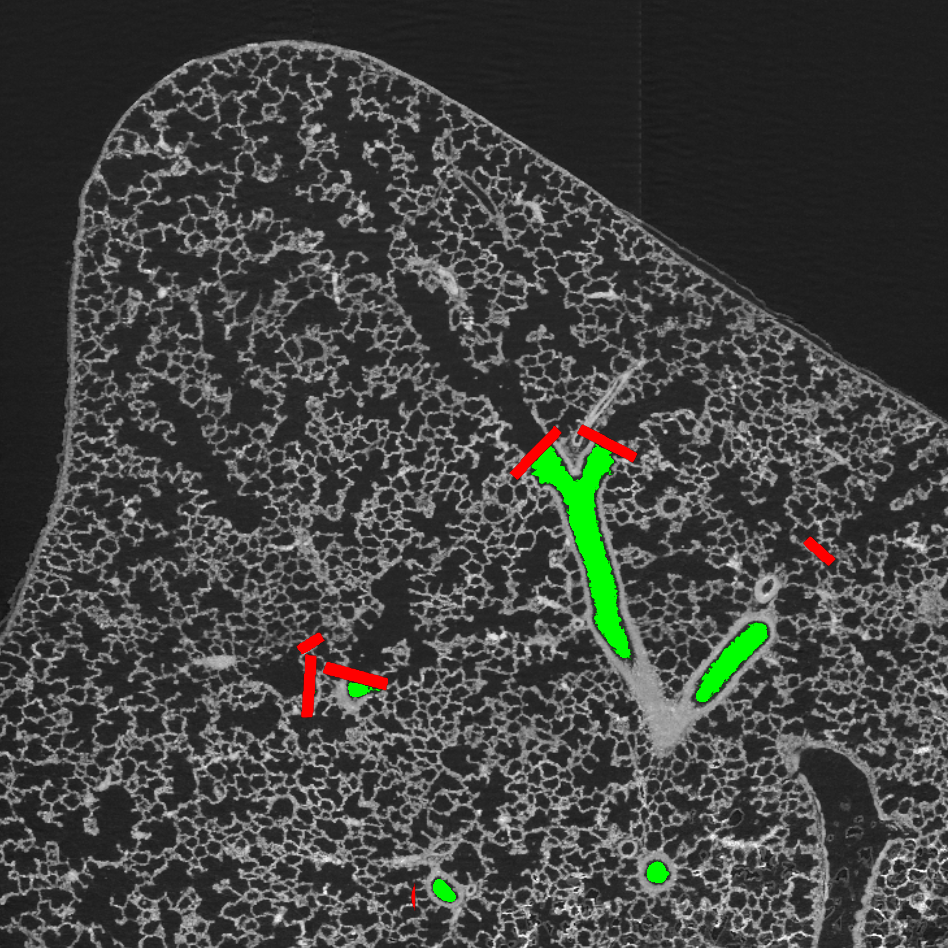
\includegraphics[width=\imagewidth]{img/ManholeCoverExplanation/60B_sagittal_slice_415}};
		% 948px = 1.403mm > 100px = 148um > 338px = 500um, 68px = 100um
		\draw[|-|,white, thick] (\x,\y) -- (\x+338,\y) node [midway, above] {\SI{500}{\micro\meter}};
		\filldraw[yellow,dashed,ultra thick, fill opacity=0.2](508,436) circle (20);
		\filldraw[yellow,dashed,ultra thick, fill opacity=0.2] (617,407) circle (20);
		\filldraw[yellow,dashed,ultra thick, fill opacity=0.2](642,434) circle (20);
		\filldraw[yellow,dashed,ultra thick, fill opacity=0.2](385,663) circle (20);
		\filldraw[yellow,dashed,ultra thick, fill opacity=0.2](347,653) circle (15);
		\filldraw[yellow,dashed,ultra thick, fill opacity=0.2] (245,667) circle (20);
		\node at (537+\s,451+\s) {1};
		\node [white] at (537,451) {1};
		\node at (606+\s,443+\s) {2};
		\node [white] at (606,443) {2};
		\node at (308+\s,683+\s) {3};
		\node [white] at (308,683) {3};
		\node at (353+\s,674+\s) {4};
		\node [white] at (353,674) {4};
		\node at (818+\s,550+\s) {5};
		\node [white] at (818,550) {5};
		\node at (309+\s,643+\s) {6};
		\node [white] at (309,643) {6};
	\end{tikzpicture}%
	\caption{Sagittal slice of one tomographic dataset showing extracted conducting airways in green and several manhole covers in red.
		The dashed yellow circles highlight some examples of alveoli which mark the change from conducting to gas-exchanging regions.
		Changes in thickness and structure of the epithelium and of the wall itself were also used to identify the entrances of the acini.
		Four segmentation stoppers (red) are shown cut right through the middle (\numrange{1}{4}), two of them are only partially cut in this slice and thus appear much smaller (5 \& 6).}
	\label{fig:ManholeCoverExplanation}
\end{figure*}

Once all acinar entrance points were defined, we extracted the volume of each isolated acinus (shown as yellow volumes in \autoref{subfig:extracted acini}) in an automated third step.
The manhole covers were defined by their diameter and surface normal.

We extracted the volume of the individual acini using an additional region growing module.
A point along the surface normal defining the manhole cover was used as seed point for this region growing segmentation.
The only manual work needed for the final extraction of the volume of each acinus was the iterative selection of the appropriate segmentation threshold and subsequent tabulation of the automatically calculated acinar volume.

\renewcommand{\imsize}{0.33\textwidth}%
\pgfmathsetlength{\imagewidth}{\imsize}%
\pgfmathsetlength{\imagescale}{\imagewidth/800}%
\def\x{55}
\def\y{745}
\begin{figure*}
	\centering
	\subfloat[Sample]{%
		\begin{tikzpicture}[x=\imagescale,y=-\imagescale]
			\node[anchor=north west, inner sep=0pt, outer sep=0pt] at (0,0) {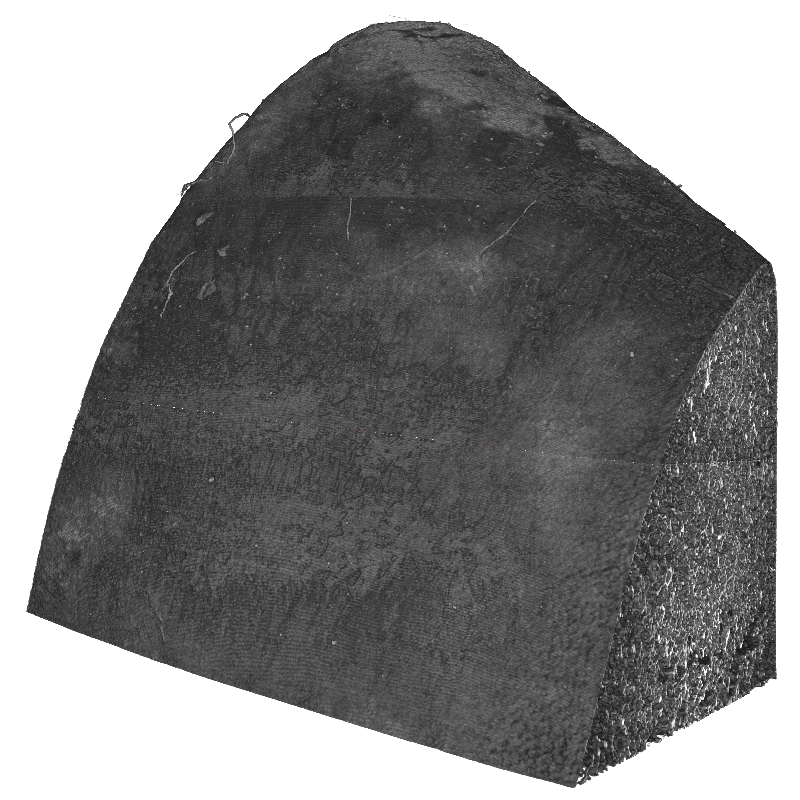
\includegraphics[width=\imagewidth]{img/ManholeCover/R108C60B_2010c_Sample}};
			% 570px = 4.363mm > 100px = 765um > 65px = 500um, 13px = 100um
			\draw[|-|,thick] (\x,\y) -- (\x+65,\y) node [right] {\SI{500}{\micro\meter}};
			\draw[dashed,green,thick] (777,460) -- (662,466) -- (84,394);
			\draw[dashed,green,thick] (723,223) -- (181,201);
		\end{tikzpicture}%
		\label{subfig:sample}%
		}%
	\subfloat[Extracted conducting airways with manhole covers shown overlaid over Sample.]{%
		\begin{tikzpicture}[x=\imagescale,y=-\imagescale]
			\node[anchor=north west, inner sep=0pt, outer sep=0pt] at (0,0) {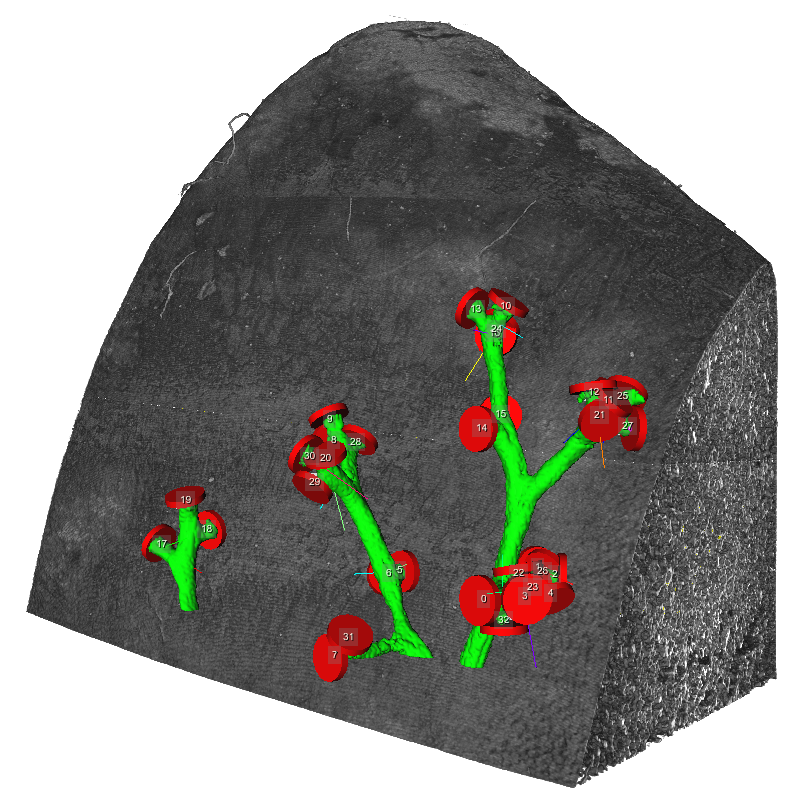
\includegraphics[width=\imagewidth]{img/ManholeCover/R108C60B_2010c_Sample_Airway}};
			% 570px = 4.363mm > 100px = 765um > 65px = 500um, 13px = 100um
			%\draw[|-|,thick] (\x,\y) -- (\x+65,\y) node [right] {\SI{500}{\micro\meter}};
		\end{tikzpicture}%
		\label{subfig:airway segment}%
		}%
	\subfloat[Extracted acini.]{%
		\begin{tikzpicture}[x=\imagescale,y=-\imagescale]
			\node[anchor=north west, inner sep=0pt, outer sep=0pt] at (0,0) {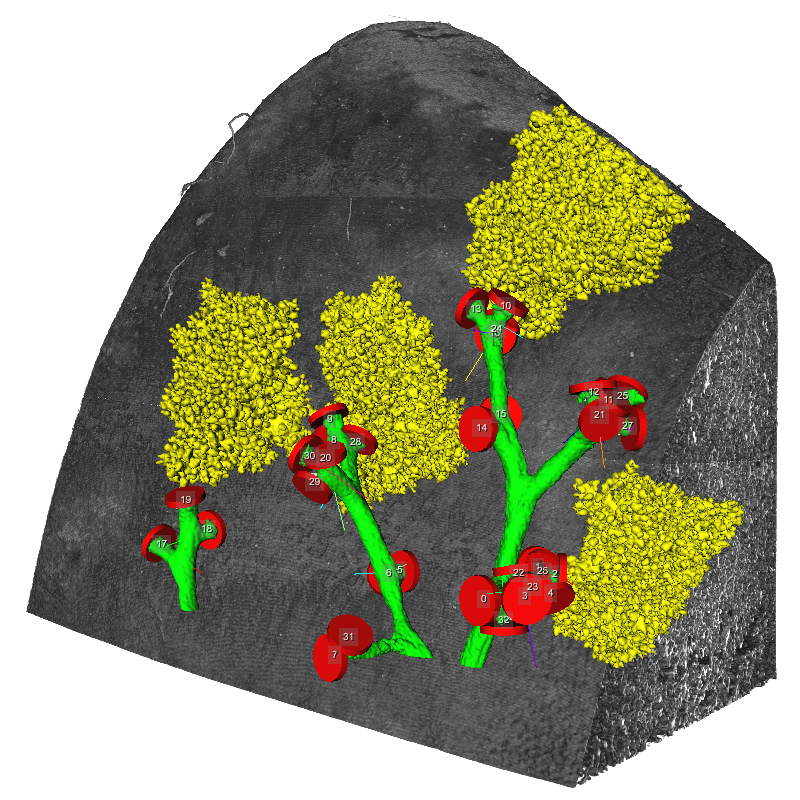
\includegraphics[width=\imagewidth]{img/ManholeCover/R108C60B_2010c_Sample_Acini}};
			%\draw[|-|,thick] (\x,\y) -- (\x+65,\y) node [right] {\SI{500}{\micro\meter}};
		\end{tikzpicture}%
		\label{subfig:extracted acini}%
		}%
	\caption{%
		Visualization of the work flow for the extraction of the acinar volumes in a rat lung sample (postnatal day 60): %
		\protect\subref{subfig:sample}: Three-dimensional visualization of the sample.
		To increase the field of view a stack of three wide field scans were taken.
		The borders between the three stacked scans are indicated by a dashed green line.
		\protect\subref{subfig:airway segment} Extracted airway segment (green) superimposed on the sample.
		Using a grey level threshold based region growing algorithm , we extracted conducting airways inside the sample.
		The red discs (nicknamed manhole covers) were semiautomatically placed and used as segmentation stoppers for the region growing during segmentation of individual acini.
		\protect\subref{subfig:extracted acini} Four extracted acini are shown superimposed over the sample in yellow.
	}
	\label{fig:workflow}
\end{figure*}

The volume of \replaced[id=dh]{each}{the} individual \replaced[id=st]{acinus}{acini} was calculated by multiplying the amount of segmented voxels by the voxel volume.
The individual acini were exported to DICOM files for further processing as described below.
The exported files contained a combination of the segmented acinar volume in the foreground with the corresponding region of interest of the original tomographic dataset in the background, as seen in \autoref{fig:STEPanizer David}.

\subsection{Stereological Analysis}
\label{sec:stereological analysis}
To check the calculated volumes against a gold standard method, we stereologically estimated the volume of the individual acini (\autoref{fig:STEPanizer David}).
To guarantee accurate and unbiased results, we standardized each step of tissue fixation, processing \added[id=st]{and} sampling\replaced[id=st]{. We performed a}{ and analysis and performed the} stereological estimation \added[id=st]{of standard lung parameters} according to \citet{Hsia2010}.

A MATLAB\textsuperscript{\textregistered} script was used to perform a systematic random sampling of slices of each individual acinus and to export the selected slices as JPG sequences for stereological analysis.

Using the web-based stereology freeware STEPanizer~\cite[\url{http://stepanizer.com}]{Tschanz2011} we analyzed the volume, surface area and number of alveoli of the extracted acini.
\added[id=st]{The volume was estimated according to the Cavalieri principle: profile area on equidistant serial sections of acini was estimated by simple point cointing.
The volume was calculated by multiplying the area estimate by the distance of the serial sections.}
Intersection\added[id=st]{ count}s of the acinar surface with geometric line probes were counted to estimate the \added[id=st]{internal} acinar surface \added[id=st]{area} (\autoref{fig:STEPanizer David})\deleted[id=st]{, while simple point counting was used to estimate the volume of the extracted acini.}
Alveolar number was estimated by counting the number of entrance rings in paired sections by using the disector\replaced[id=st]{~\cite{Sterio1984} accomplished with the STEPanizer (experimental feature).}{mode of the STEPanizer~\citep{Hsia2010}} (\autoref{fig:STEPanizer Evelyne}).

\renewcommand{\imsize}{\linewidth}%
\pgfmathsetlength{\imagewidth}{\imsize}%
\pgfmathsetlength{\imagescale}{\imagewidth/1280}%
\pgfmathsetlength{\imagescale}{\imagewidth/1280}%
\begin{figure}[htb]
	\centering
	\begin{tikzpicture}[x=\imagescale,y=-\imagescale]
		\node[anchor=north west, inner sep=0pt, outer sep=0pt] at (0,0) {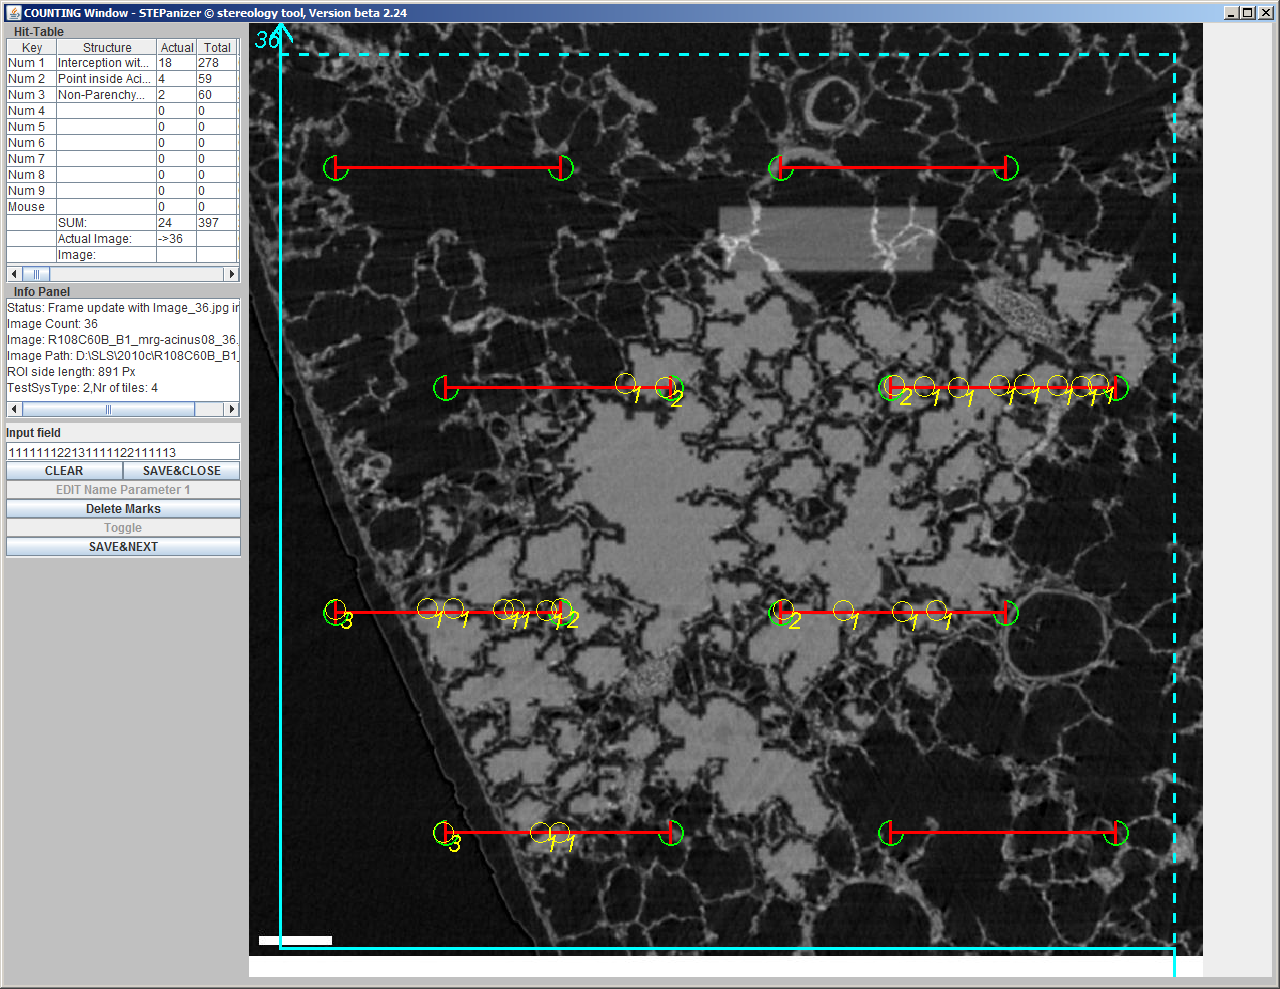
\includegraphics[width=\imagewidth]{img/STEPanizer_2010_R108C60B_acinus08_Slice36}};
		% 914px = 0.1mm > 100px = 11um > 4568px = 500um, 914px = 100um
		\draw[dashed,green,thick] (719,207) -- (937,207) -- (932,270) -- (723,270) -- cycle ;
	\end{tikzpicture}%
	\caption{Screenshot from the STEPanizer counting window.
		The segmented acinus is visible in light grey, the manhole cover which was used to separate this acinus is marked with a dashed green line.
		Both structures have been merged with the original tomographic data using our MeVisLab work flow and exported to a stack of JPG files.
		Line and point probes used for counting are shown as red lines and green circles.
		Counting events are marked as yellow circles.
		Scale bar: \SI{100}{\micro\meter}.}
	\label{fig:STEPanizer David}
\end{figure}

\renewcommand{\imsize}{\linewidth}
\begin{figure}[htb]
	\centering
	\subfloat[Disector mode, Image a: sampling]{%
		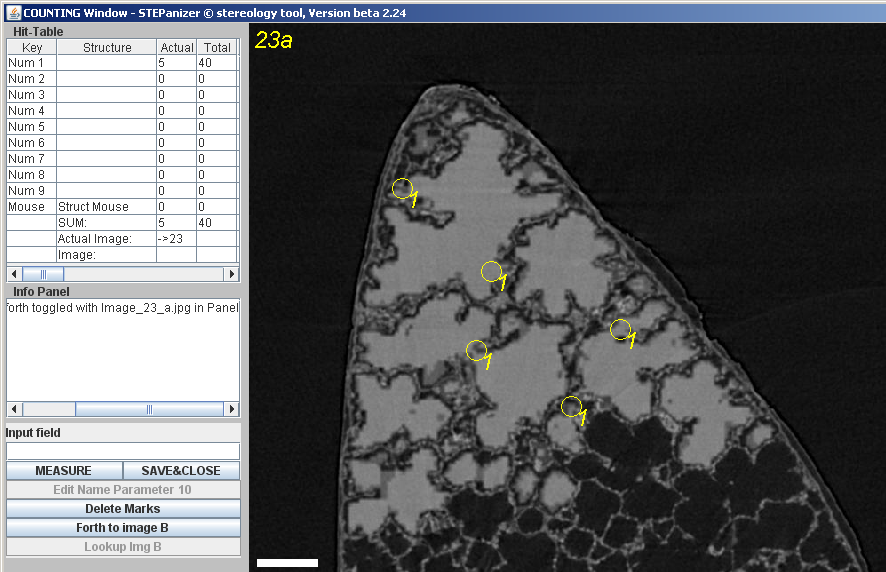
\includegraphics[width=\imsize]{img/R108C60B_B1_mrg-acinus10_EntranceCountingA_crop_edit}%
		\label{subfig:sampling}%
		}\\
	\subfloat[Disector mode, Image b: look-up]{%
		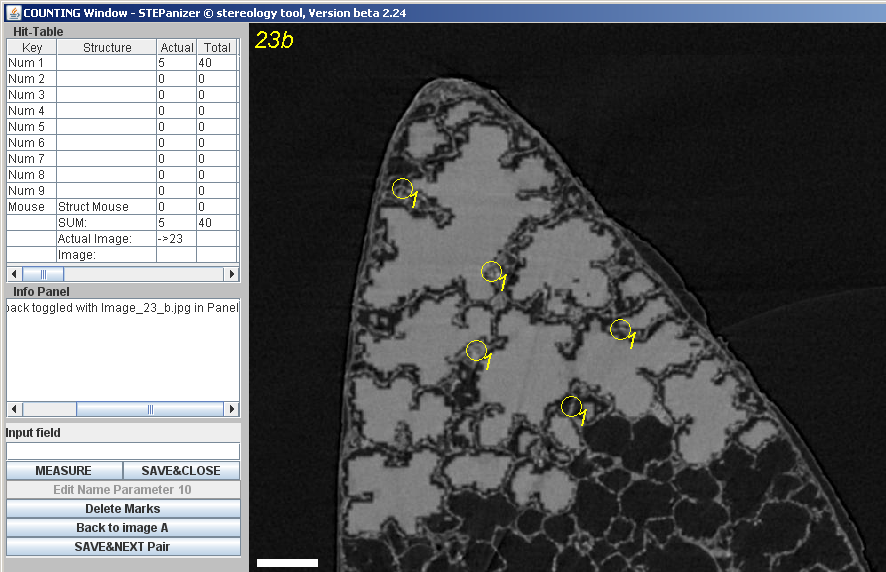
\includegraphics[width=\imsize]{img/R108C60B_B1_mrg-acinus10_EntranceCountingB_crop_edit}%
		\label{subfig:lookup}%
		}
	\caption{Screenshots from the STEPanizer counting window in disector mode.
		The segmented acinus is visible in light grey, appearing and disappearing bridges corresponding to alveolar entrance rings are counted and marked by yellow circles.
		Scale bar: \SI{100}{\micro\meter}.}
	\label{fig:STEPanizer Evelyne}
\end{figure}

\section{Results}
\label{sec:results}
\subsection{Segmentation of individual acini}
The novel method described in \autoref{sec:manhole covers} was used to extract individual functional units of three rat lungs from high resolution synchrotron radiation based tomographic datasets.
Based on morphological criteria (thickness of the wall of the airways and appearance of the most distal alveoli) we place segmentation stopper into the airways at the transition of purely conducting to gas-exchanging airways (\autoref{fig:ManholeCoverExplanation}).
As a result we were able to isolate individual acini (two acini are shown in \autoref{fig:acini}).
\deleted[id=st,remark=redundant]{We nicknamed the segmentation stoppers manhole cover.}
In the next step we performed a segmentation of \numberofacini individual acini (see \autoref{tab:results}) using a grey level threshold based region growing algorithm.

\deleted[id=st,remark={moved to discussion}]{To our best knowledge, an extraction of such a high number of rat lung acini from high resolution tomographic datasets has never been achieved before.
It enabled us to obtain statistical data on acinar volume, surface area and numbers of alveoli per acinus.}

\subsection{Acinar volume}
The volume of individual acini was either automatically assessed by adding the segmented voxels inside the acini and multiplying them with the voxel volume or manually estimated by using the Cava\deleted[id=sb]{g}lieri method~\replaced[id=st]{\citep{Cruz-Orive1999}}{\citep{Hsia2010}}.

A mean \added[id=sb]{acinar} volume of \SI{\meanacinarvolume}{\milli\meter\cubed} and a standard deviation of \SI{\meanacinarvolumeSTD}{\milli\meter\cubed} was estimated (see \autoref{tab:results} for details).
We removed 4 outliers from the volume data because their value was larger than the mean volume value \(\pm\biggerthan\times\) standard deviation (red dots in \autoref{fig:Volume plots}).

\renewcommand{\imsize}{0.33\linewidth}
\begin{figure*}[htb]
	\centering
	\subfloat[Acinus 10, location in sample]{%
		\pgfmathsetlength{\imagewidth}{\imsize}%
		\pgfmathsetlength{\imagescale}{\imagewidth/701}%
		\def\x{55}% scalebar-x at golden ratio of x=701px
		\def\y{721}% scalebar-y at 90% of height of y=801px
			\begin{tikzpicture}[x=\imagescale,y=-\imagescale]
				\clip (0,0) rectangle (701,801);
				\node[anchor=north west, inner sep=0pt, outer sep=0pt] at (0,0) {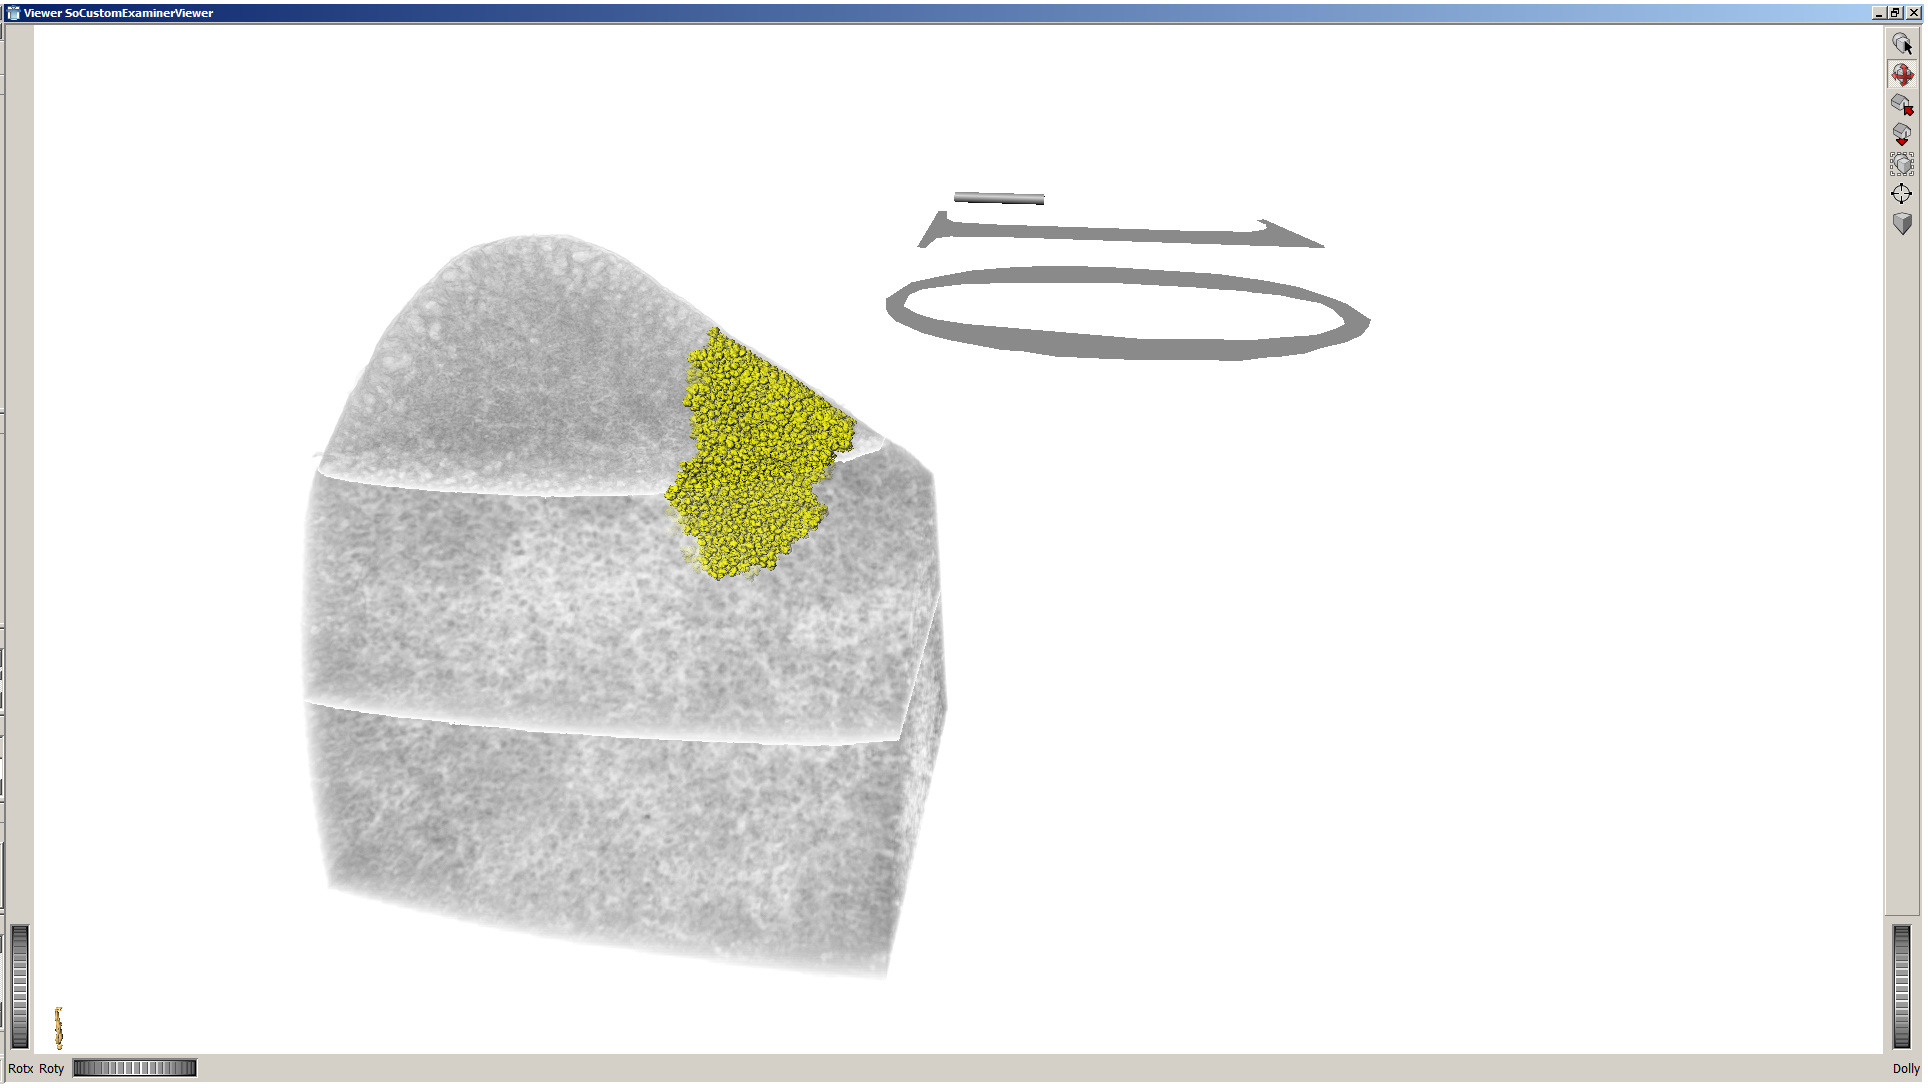
\includegraphics[width=\imagewidth]{img/SingleAcinusFullView/acinus10_01}};
				\draw[|-|,thick] (\x,\y) -- (\x+65,\y) node [right] {\SI{500}{\micro\meter}};
\end{tikzpicture}%
		}%
	\subfloat[Acinus 10, view 1]{%
		\pgfmathsetlength{\imagewidth}{\imsize}%
		\pgfmathsetlength{\imagescale}{\imagewidth/718}%
			\begin{tikzpicture}[x=\imagescale,y=-\imagescale]
				\clip (0,0) rectangle (718,576);
				\node[anchor=north west, inner sep=0pt, outer sep=0pt] at (0,0) {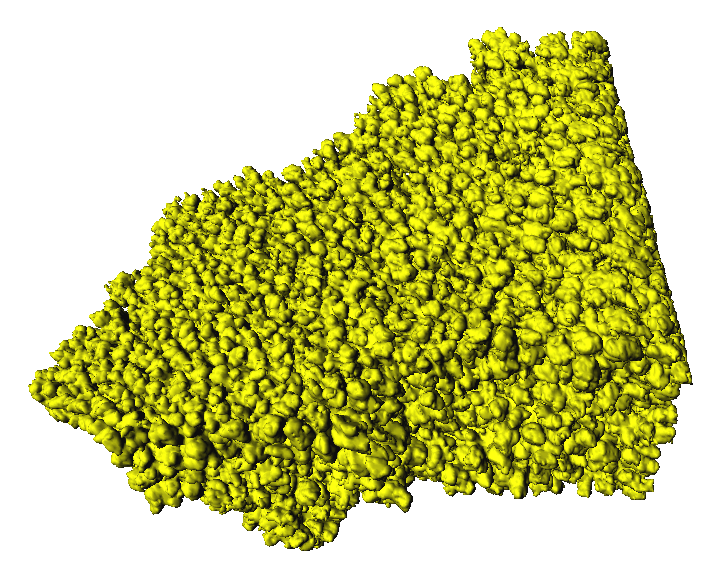
\includegraphics[width=\imagewidth]{img/SingleAcinusFullView/acinus10_03}};
				\draw[red, semitransparent, ultra thick, rotate around={-5:(340,428)}] (340,428) ellipse (70 and 20);
			\end{tikzpicture}%
		}%
	\subfloat[Acinus 10, view 2]{%
		\pgfmathsetlength{\imagewidth}{\imsize}%
		\pgfmathsetlength{\imagescale}{\imagewidth/1169}%
			\begin{tikzpicture}[x=\imagescale,y=-\imagescale]
				\clip (0,0) rectangle (1169,959);
				\node[anchor=north west, inner sep=0pt, outer sep=0pt] at (0,0) {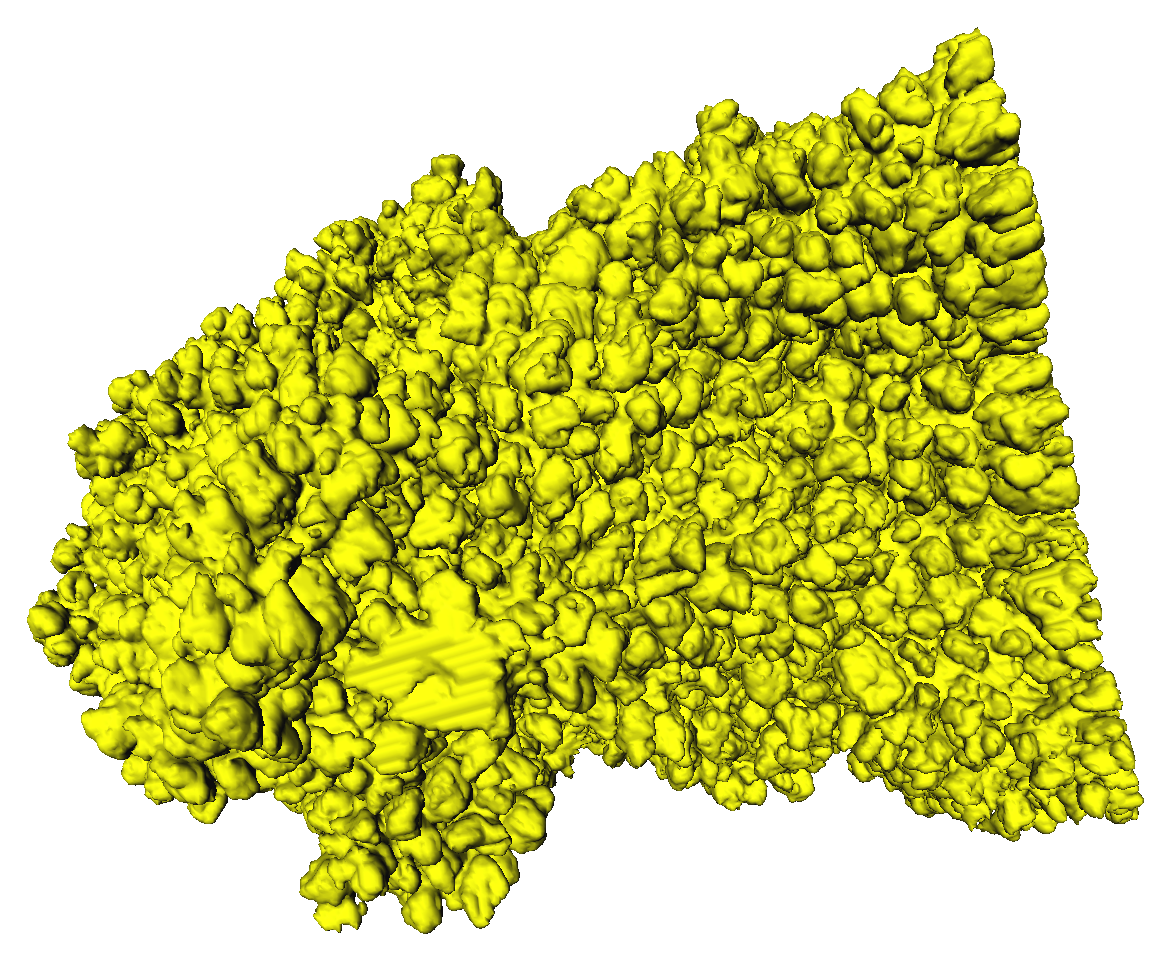
\includegraphics[width=\imagewidth]{img/SingleAcinusFullView/acinus10_04}};
				\draw[red, semitransparent, ultra thick] (422,647) ellipse (115 and 80);
			\end{tikzpicture}%
		}%
	\\%
	\subfloat[Acinus 26, location in sample]{%
		\pgfmathsetlength{\imagewidth}{\imsize}%
		\pgfmathsetlength{\imagescale}{\imagewidth/833}%
		\def\x{55}% scalebar-x at golden ratio of x=833px
		\def\y{756}% scalebar-y at 90% of height of y=840px
			\begin{tikzpicture}[x=\imagescale,y=-\imagescale]
				\clip (0,0) rectangle (833,840);
				\node[anchor=north west, inner sep=0pt, outer sep=0pt] at (0,0) {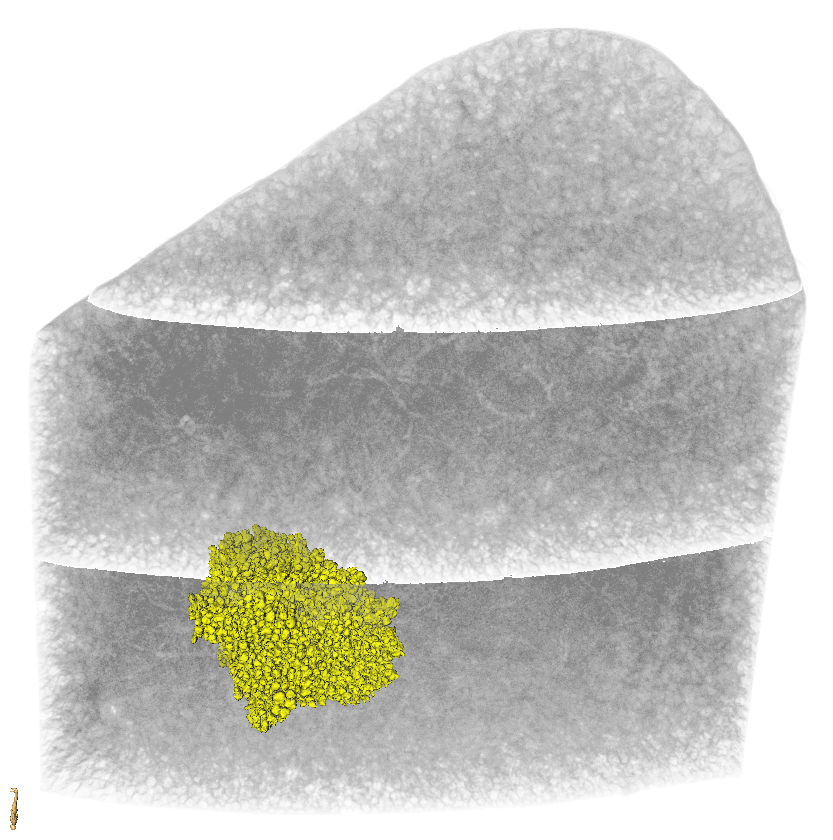
\includegraphics[width=\imagewidth]{img/SingleAcinusFullView/acinus26_07}};
				% 702px = 4.363mm > 100px = 621um > 80px = 500um, 16px = 100um
				%\draw[|-|,blue,thick] (40,791) -- (742,775) node [sloped,midway,above,fill=white,semitransparent,text opacity=1] {\SI{4.363}{\milli\meter} (2948px)};
				\draw[|-|,thick] (\x,\y) -- (\x+80,\y) node [right] {\SI{500}{\micro\meter}};
			\end{tikzpicture}%
		}%
	\subfloat[Acinus 26, view 1]{%
		\pgfmathsetlength{\imagewidth}{\imsize}%
		\pgfmathsetlength{\imagescale}{\imagewidth/1089}%
			\begin{tikzpicture}[x=\imagescale,y=-\imagescale]
				\clip (0,0) rectangle (1089,880);
				\node[anchor=north west, inner sep=0pt, outer sep=0pt] at (0,0) {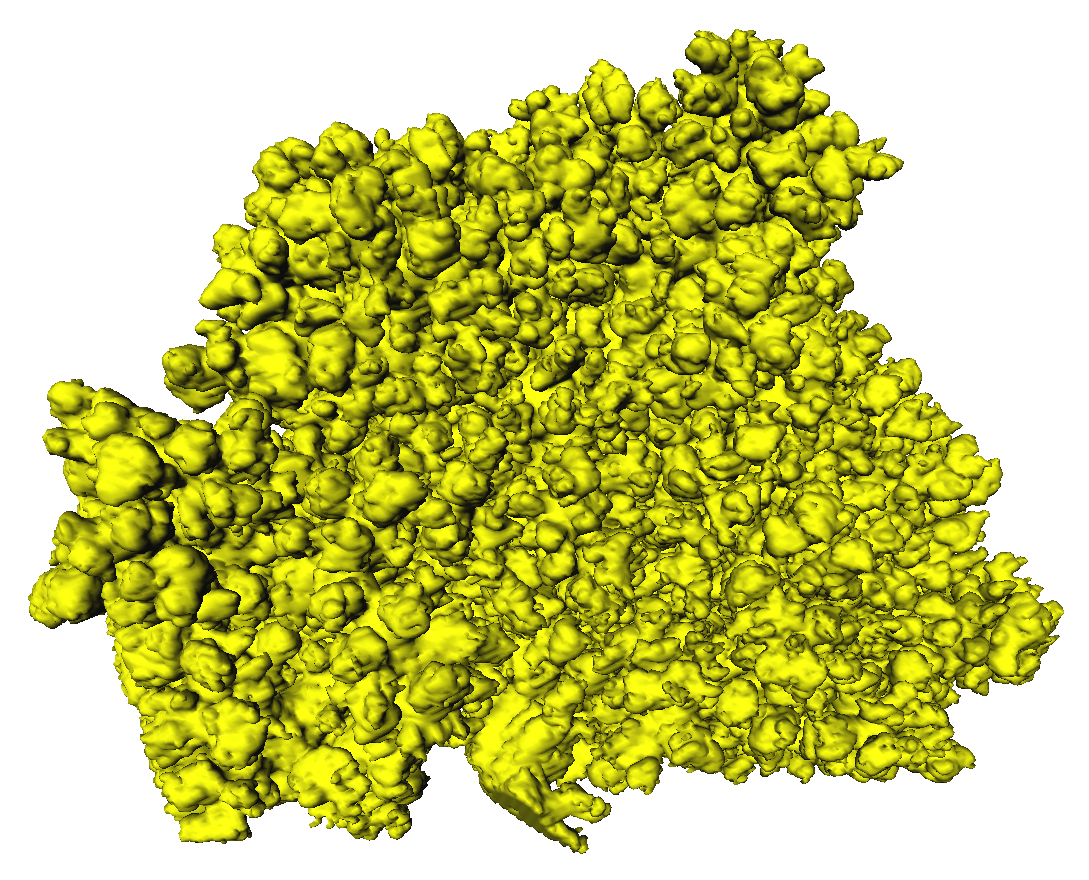
\includegraphics[width=\imagewidth]{img/SingleAcinusFullView/acinus26_11}};
				\draw[red,semitransparent,ultra thick, rotate around={-40:(524,802)}] (524,802) ellipse (70 and 40);
			\end{tikzpicture}%
		}%
	\subfloat[Acinus 26, view 2]{%
		\pgfmathsetlength{\imagewidth}{\imsize}%
		\pgfmathsetlength{\imagescale}{\imagewidth/839}%
			\begin{tikzpicture}[x=\imagescale,y=-\imagescale]
				\clip (0,0) rectangle (830,953);
				\node[anchor=north west, inner sep=0pt, outer sep=0pt] at (0,0) {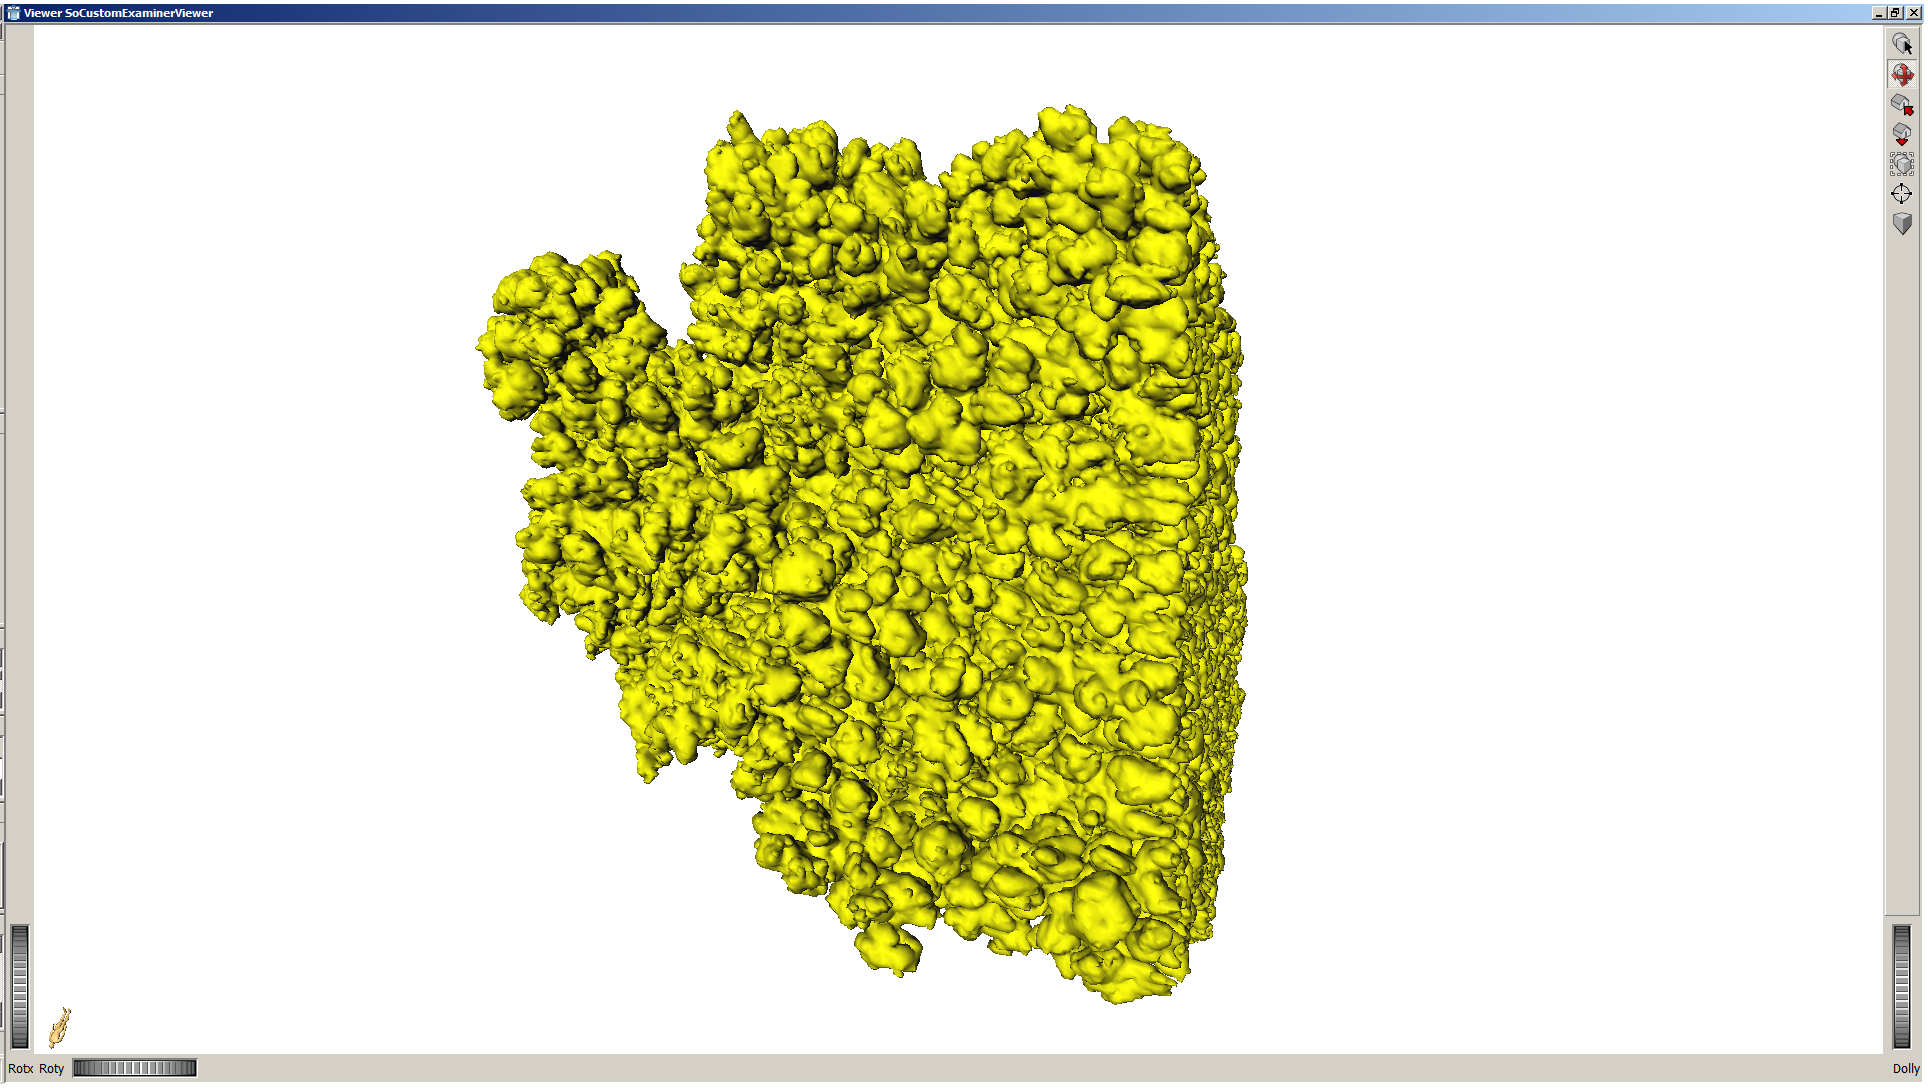
\includegraphics[width=\imagewidth]{img/SingleAcinusFullView/acinus26_13}};
			\end{tikzpicture}%
		}%
	\caption{Views of two rat acini.
		Left: Location of the acinus inside the sample.
		Middle and right: two different views of each acinus.
		The red circles mark the approximate position of the segmentation stopper, when visible.
		Movies of the two acini are in the supporting material, available online.}
	\label{fig:acini}
\end{figure*}

\subsection{Acinar surface area}\label{sec:results:acinar surface area}
The estimation of a surface area \added[id=st]{, which corresponds to the diffusion relevant gas exchange surface,} causes the classic coastline paradox where a measurement of a length or surface area heavily depends on the scale of the measurement~\citep{Mandelbrot1967a}.
To automatically extract the surface area of the individual acini one would need to perform a three-dimensional triangulation of the alveolar surface by mapping the edges of voxels to adjoining triangles in the three-dimensional space.
While various methods of triangulating a surface do exist, limitations in our computing power would have required a binning of the data which represents a reduction of the resolution.

There are several methods for triangulation of three-dimensional surfaces~\citep{Lorensen1987, Schneiders1996}, nonetheless all these methods cannot overcome the problem of the coastline paradox.
We thus did not assess the acinar surface by triangulation (\eg using MeVisLab).

Instead of the triangulation method, we preferred a classical stereological to estimate the surface area of the acini by counting interception of test lines with the alveolar septa~\citep{Hsia2010} at the original resolution of our datasets, which was approximately equal to light microscopical images take with a \(10\times\) lens.

For the three different animals we calculated a mean acinar surface of \SI{\meanacinarsurface}{\milli\meter\squared} with a standard deviation of \meanacinarsurfaceSTD (see \autoref{tab:results} for details).

\subsection{Number of alveoli per acinus}
\replaced[id=st]{By applying the disector principle we counted the new appearance of alveolar entrance rings corresponding to the number of alveoli (Hyde 20xx, Ochs, 20xx).
In practice the presence or absence of a tissue bridge connecting the free edges of alveolar septa on one section}{By counting the presence or absence of a bridge connecting the free edges of alveolar septa on one image} (sampling, \autoref{subfig:sampling}) but not on the other \added[id=st]{one} (look-up, \autoref{subfig:lookup}) \replaced[id=st]{is counted. W}{, w}e found a mean number of alveoli for all analyzed acini of \meannumberofalveoli with a standard deviation of \meannumberofalveoliSTD (see \autoref{tab:results} for details).

\subsection{Total number of acini}\label{sec:results:total number of acini}
We estimated \replaced[id=st]{the}{an} total number of acini per lung by dividing the total parenchymal volume by the mean acinar volume.
For the three lung investigated we calculated \totalnumberofaciniB, \totalnumberofaciniD and \totalnumberofaciniE acini per lung, respectively, resulting in a mean of \meantotalnumberofacini with a standard deviation of \meantotalnumberofaciniSTD.

The absolute number of acini per lung can also be estimated by dividing the estimated total number of alveoli \added[id=st]{in the entire lung} (\added[id=dh]{calculated on based on} personal communication Stefan Tschanz and Johannes Schittny) by the number of alveoli per acinus.
For the three lung investigated we calculated \totalnumberofaciniBVariant, \totalnumberofaciniDVariant and \totalnumberofaciniEVariant acini per lung, respectively, resulting in a mean of \meantotalnumberofaciniVariant with a standard deviation of \meantotalnumberofaciniSTDVariant.

\begin{table*}[htb]
	\centering
	\caption{Summary of results}
	\noindent\makebox[\textwidth]{
	\begin{tabular}{p{0.3\linewidth}ccccc}
	\toprule
																	& Animal 1 							& Animal 2 							& Animal 3 							& Mean 									& Standard Deviation \\
	\midrule
	Number of analyzed acini 									& \numberofaciniB 					& \numberofaciniD					& \numberofaciniE 					& 											& \\
	Acinar volume [\si{\milli\meter\cubed}]				& \acinarvolumeB 					& \acinarvolumeD					& \acinarvolumeE 					& \meanacinarvolume 					& \meanacinarvolumeSTD \\
	Acinar surface [\si{\milli\meter\squared}]			& \acinarsurfaceB 					& \acinarsurfaceD 					& \acinarsurfaceE					& \meanacinarsurface 					& \meanacinarsurfaceSTD \\
	Alveoli per acinus 											& \numberofalveoliB 				& \numberofalveoliD 				& \numberofalveoliE					& \meannumberofalveoli 				& \meannumberofalveoliSTD \\
	Total number of acini (surface based calculation)	& \totalnumberofaciniB 			& \totalnumberofaciniD 			& \totalnumberofaciniE 			& \meantotalnumberofacini 			& \meantotalnumberofaciniSTD \\
	Total number of acini (alveoli based calculation)	& \totalnumberofaciniBVariant 	& \totalnumberofaciniDVariant 	& \totalnumberofaciniEVariant	& \meantotalnumberofaciniVariant 	& \meantotalnumberofaciniSTDVariant \\
	\bottomrule
	\end{tabular}
	}
	\label{tab:results}
\end{table*}

\subsection{Comparison of Volumes from \replaced[id=st]{automatic vs.\ manual assessment}{MeVisLab with STEPanizer}}
The volume of the individual \added[id=sb]{acinus} has been assessed by automatic voxel counting (\autoref{sec:manhole covers}) as well as by manual, stereological estimation (\autoref{sec:stereological analysis}).

The manual stereological method results in a value \(\difference\times\) larger than the automatic method using voxel counting.
Detailed results are shown in \autoref{fig:Volume plots} and \added[id=st]{the considerable difference} explained later on in \replaced[id=dh]{the Discussion}{section \ref{sec:discussion}}.
Values larger than the mean of the volumes \(\pm\biggerthan\times\) the standard deviation have been removed from the calculation (red dots).

\renewcommand{\imsize}{0.35\textwidth}
\begin{figure*}[htb]
	\centering
	\subfloat{
		\begin{tikzpicture}

\begin{axis}[
	width=\imsize,
	xlabel={Acinus},
	ylabel={Volume [\si{\milli\meter\cubed}]},
	ymin=1e-7, ymax=4,
	scaled ticks=true,
	%yticklabel=\empty
	]
\addplot [red, only marks]
coordinates {
(0,0.37731293) (1,0.19965522) (2,0.25447792) (3,0.43383464) (4,nan) (5,0.31837037) (6,0.42459121) (7,nan) (8,0.294278) (9,0.26970762) (10,0.47316542) (11,0.13395399) (12,0.2331105) (13,nan) (14,0.66745716) (15,0.45502964) (16,nan) (17,nan) (18,0.47915584) (19,nan) (20,0.43513966) (21,0.33121431) (22,0.15090302) (23,nan) (24,0.14413643) (25,nan) (26,0.24587891) (27,0.27121842) (28,0.16399051) (29,0.38648456) (30,0.32862523) (31,0.19227928) 
};
\addplot [green, only marks]
coordinates {
(0,0.37731293) (1,0.19965522) (2,0.25447792) (3,0.43383464) (4,nan) (5,0.31837037) (6,0.42459121) (7,nan) (8,0.294278) (9,0.26970762) (10,0.47316542) (11,0.13395399) (12,0.2331105) (13,nan) (14,nan) (15,0.45502964) (16,nan) (17,nan) (18,0.47915584) (19,nan) (20,0.43513966) (21,0.33121431) (22,0.15090302) (23,nan) (24,0.14413643) (25,nan) (26,0.24587891) (27,0.27121842) (28,0.16399051) (29,0.38648456) (30,0.32862523) (31,0.19227928) 
};
\addplot [cyan]
	coordinates {
		(0,0.304196244782609) (32,0.304196244782609)
	};
\addplot [cyan, dashed]
	coordinates {
		(0,0.634325534516513) (32,0.634325534516513) 
	};
\addplot [cyan, dashed]
	coordinates {
		(0,-2.59330449512958e-02) (32,-2.59330449512958e-02) 
	};

\end{axis}

\end{tikzpicture}%
		}\hfill%
	\subfloat{
		\begin{tikzpicture}

\begin{axis}[
	width=\imsize,
	xlabel={Acinus},
	%ylabel={Volume [\si{\centi\meter\cubed}]},
	ymin=1e-7, ymax=4,
	]
\addplot [red, only marks]
coordinates {
(0,nan) (1,nan) (2,nan) (3,0.5900293) (4,0.55371433) (5,nan) (6,nan) (7,0.29986489) (8,nan) (9,0.39014131) (10,0.29307008) (11,nan) (12,nan) (13,nan) (14,nan) (15,0.42841768) (16,nan) (17,nan) (18,0.4532719) (19,0.23229824) (20,nan) (21,nan) (22,nan) (23,0.58026904) (24,nan) (25,nan) (26,0.51905155)
};
\addplot [green, only marks]
coordinates {
(0,nan) (1,nan) (2,nan) (3,0.5900293) (4,0.55371433) (5,nan) (6,nan) (7,0.29986489) (8,nan) (9,0.39014131) (10,0.29307008) (11,nan) (12,nan) (13,nan) (14,nan) (15,0.42841768) (16,nan) (17,nan) (18,0.4532719) (19,0.23229824) (20,nan) (21,nan) (22,nan) (23,0.58026904) (24,nan) (25,nan) (26,0.51905155)
};
\addplot [cyan]
	coordinates {
		(0,0.434012832) (27,0.434012832) 
	};
\addplot [cyan, dashed]
	coordinates {
		(0,0.79918601656343) (27,0.79918601656343) 
	};
\addplot [cyan, dashed]
	coordinates {
		(0,6.88396474365702e-02) (27,6.88396474365702e-02) 
	};

\end{axis}

\end{tikzpicture}
		}\hfill%
	\subfloat{
		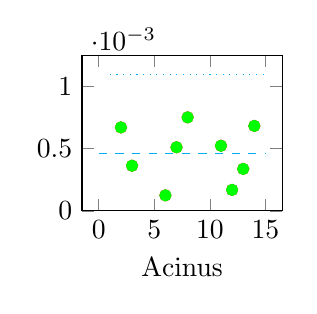
\begin{tikzpicture}

\begin{axis}[
	width=0.34*\linewidth,
	xlabel={Acinus},
	%ylabel={Volume [\si{\centi\meter\cubed}]},
	ymin=1e-7, ymax=1.25e-3,
	]
\addplot [red, only marks]
coordinates {
(0,nan) (1,nan) (2,0.0006709888) (3,0.00036325091) (4,nan) (5,nan) (6,0.00012486846) (7,0.00051163185) (8,0.00075202513) (9,nan) (10,nan) (11,0.00052375108) (12,0.00016866906) (13,0.00033741882) (14,0.00068318522)
};
\addplot [green, only marks]
coordinates {
(0,nan) (1,nan) (2,0.0006709888) (3,0.00036325091) (4,nan) (5,nan) (6,0.00012486846) (7,0.00051163185) (8,0.00075202513) (9,nan) (10,nan) (11,0.00052375108) (12,0.00016866906) (13,0.00033741882) (14,0.00068318522)
};
\addplot [cyan, dashed]
	coordinates {
		(0,0.000459532147777778) (15,0.000459532147777778) 
	};
\addplot [cyan, dotted]
	coordinates {
		(1,0.00109820895859664) (15,0.00109820895859664) 
	};
\addplot [cyan, dotted]
	coordinates {
		(1,-0.000179144663041085) (15,-0.000179144663041085) 
	};

\end{axis}

\end{tikzpicture}
		}\\%
	\subfloat{
		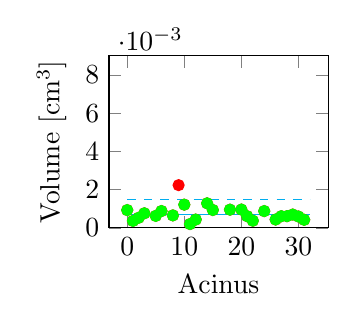
\begin{tikzpicture}

\begin{axis}[
	width=0.36*\linewidth,
	xlabel={Acinus},
	ylabel={Volume [\si{\centi\meter\cubed}]},
	ymin=1e-7, ymax=0.009,
	%ymin=0, ymax=0.0042,
	%yticklabel=\empty
	]
\addplot [red, only marks]
coordinates {
(0,0.000928503038942363) (1,0.000363236072194969) (2,0.000528476198612276) (3,0.000761414474783716) (4,nan) (5,0.000626766920809997) (6,0.000878359350940617) (7,nan) (8,0.000651206767483189) (9,0.00223488663353551) (10,0.00121456308634507) (11,0.000199220648894286) (12,0.000433235998567998) (13,nan) (14,0.00128366813580556) (15,0.00093334944120013) (16,nan) (17,nan) (18,0.000951931319014455) (19,nan) (20,0.000957101812399371) (21,0.000611808517484639) (22,0.000373053974075999) (23,nan) (24,0.000876431577102944) (25,nan) (26,0.000435061652353202) (27,0.000608824085692031) (28,0.000611808517484639) (29,0.000695108832432261) (30,0.000592133625582743) (31,0.000420831138489319) 
};
\addplot [green, only marks]
coordinates {
(0,0.000928503038942363) (1,0.000363236072194969) (2,0.000528476198612276) (3,0.000761414474783716) (4,nan) (5,0.000626766920809997) (6,0.000878359350940617) (7,nan) (8,0.000651206767483189) (9,nan) (10,0.00121456308634507) (11,0.000199220648894286) (12,0.000433235998567998) (13,nan) (14,0.00128366813580556) (15,0.00093334944120013) (16,nan) (17,nan) (18,0.000951931319014455) (19,nan) (20,0.000957101812399371) (21,0.000611808517484639) (22,0.000373053974075999) (23,nan) (24,0.000876431577102944) (25,nan) (26,0.000435061652353202) (27,0.000608824085692031) (28,0.000611808517484639) (29,0.000695108832432261) (30,0.000592133625582743) (31,0.000420831138489319) 
};
\addplot [cyan]
	coordinates {
		(0,0.000692873703769207) (32,0.000692873703769207) 
	};
\addplot [cyan, dashed]
	coordinates {
		(0,0.0015013239011447) (32,0.0015013239011447) 
	};
\addplot [cyan, dashed]
	coordinates {
		(0,-0.000115576493606282) (32,-0.000115576493606282) 
	};

\end{axis}

\end{tikzpicture}
		}\hfill%
	\subfloat{
		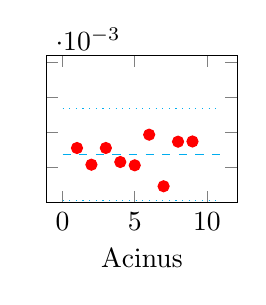
\begin{tikzpicture}

\begin{axis}[
	width=0.33*\linewidth,
	xlabel={Acinus},
	%ylabel={Volume [\si{\centi\meter\cubed}]},
	ymin=0, ymax=0.0042,
	yticklabel=\empty
	]
\addplot [red,only marks]
	coordinates {
		(1,0.00155172120433958)
		(2,0.00107560449835204)
		(3,0.00155219458912006)
		(4,0.00115221850801792)
		(5,0.0010581421745156)
		(6,0.00193194271026777)
		(7,0.000460166958864983)
		(8,0.00173206190419837)
		(9,0.0017382061817182)
	};
\addplot [cyan, dashed]
	coordinates {
		(0,0.00136136208104384) (11,0.00136136208104384) 
	};
\addplot [cyan, dotted]
	coordinates {
		(0,0.00266793742202647) (11,0.00266793742202647) 
	};
\addplot [cyan, dotted]
	coordinates {
		(0,5.47867400612025e-05) (11,5.47867400612025e-05) 
	};
\end{axis}

\end{tikzpicture}
		}\hfill%
	\subfloat{
		\begin{tikzpicture}

\begin{axis}[
	width=\imsize,
	xlabel={Acinus},
	%ylabel={Volume [\si{\centi\meter\cubed}]},
	ymin=1e-7, ymax=4,
	%yticklabel=\empty
	]
\addplot [red, only marks]
coordinates {
(0,nan) (1,nan) (2,1.80894828376899) (3,1.08657864429912) (4,nan) (5,nan) (6,0.213737862253818) (7,2.43389564249541) (8,8.8706408927333) (9,nan) (10,nan) (11,1.90254809872315) (12,0.39743256425486) (13,0.813800299917009) (14,2.45645691813613)
};	
\addplot [green, only marks]
coordinates {
(0,nan) (1,nan) (2,1.80894828376899) (3,1.08657864429912) (4,nan) (5,nan) (6,0.213737862253818) (7,2.43389564249541) (8,nan) (9,nan) (10,nan) (11,1.90254809872315) (12,0.39743256425486) (13,0.813800299917009) (14,2.45645691813613)
};
\addplot [cyan]
	coordinates {
		(0,1.38917478923106) (15,1.38917478923106) 
	};
\addplot [cyan, dashed]
	coordinates {
		(0,3.86715471927792) (15,3.86715471927792) 
	};
\addplot [cyan, dashed]
	coordinates {
		(0,-1.0888051408158) (15,-1.0888051408158) 
	};

\end{axis}

\end{tikzpicture}
		}%
	\caption{Plot of the estimated acinar volumes of each sample, extracted with MeVisLab \added[id=st]{(automatic method)} and estimated using the STEPanizer \added[id=st]{(manual assessment)}.
		The line corresponds to the mean, the dashed lines correspond to the mean \ifJCS plus or minus \biggerthan x\xspace\else\(\pm\biggerthan\times\)\xspace\fi the standard deviation.
		Red dots represent outliers and were not used for calculating the mean.
		Top row: \replaced[id=st]{Automatically assessed}{MeVisLab} volumes, bottom row: \replaced[id=st]{Manually assessed}{STEPanizer} volumes.
		From left to right: animal 1, 2 and 3.}
	\label{fig:Volume plots}
\end{figure*}


\section{Discussion}\label{sec:discussion}
An estimation of the volume, surface area as well as number of contained alveoli and septal length \replaced[id=st]{assigned to one particular acinus}{length for individual acini} is not possible using light microscopy on classic tissue sections.
\replaced[id=st]{Losing}{This is the case because} the three-dimensional context \replaced[id=st]{of a supposed acinus on sections prevents an unbiased assignment to an indivisual acinus.}{is destroyed and features on one slice cannot easily be assigned to individual acini}.

With our proposed method we \replaced[id=dh]{asdf}{asdf} can extract individual acini from three-dimensional tomographic datasets without destroying the three-dimensional context.
The three-dimensional structure of the lung samples is preserved during the tomographic imaging, we can thus extract individual acini and assess all the biologically interesting parameters mentioned above for each acinus individually.

\added[id=st,remark={moved from results}]{To our best knowledge, an extraction of such a high number of rat lung acini from high resolution tomographic datasets has never been achieved before.
\replaced[id=dh]{The extraction we performed}{It} \replaced[id=sb]{allows}{enabled} us to obtain statistical data on acinar volume, surface area and numbers of alveoli per acinus.}

The volume of the acini can be extracted automatically, parameters like surface area as well as number of contained alveoli and septal length per acinus (not shown) can be extracted with simple stereological counting, requiring manual labor.

With the proposed method we can additionally analyze structural changes in the acinus during postnatal development, like disease or differences between wild-type and knock-out animals.

\subsection{Acinar volume}
\citet{Rodriguez1987} found that the right upper lobe of one rat contains 613 acini with a mean volume of \SI{1.98}{\milli\meter\cubed} (\SIrange{0.5}{5}{\milli\meter\cubed}).
\citet{Mercer1987a} state that the total volume of \blockquote{alveoli + ducts} \eg ventilatory units is \SI{0.522(56)}{\milli\meter\cubed} (mean of 8). % http://is.gd/qpMEV5
Our calculations resulted in a volume of \SI{\meanacinarvolume}{\milli\meter\cubed} with a standard deviation of \SI{\meanacinarvolumeSTD}{\milli\meter\cubed}.
If we take in account that \citet{Mercer1987a} measured the volume of ventilatory units that have been defined differently (they define the transitory bronchioles as conducting airways, \ie their acinus is about two times smaller than our acinus), our stereologically estimated mean acinar volume is in the range of previously published data.

\subsection{Number of alveoli per acinus}
\citet{Vasilescu2012} found that the \blockquote{mean number of alveoli per acinus was 596\(\pm\)326 in the young mice and 936\(\pm\)254 in the old mice}.
Rat lungs are obviously larger than \replaced[id=st][{mouse}{mice} lungs.
Based on the strains we studied (SV 127 mice versus Sprague-Dawley rats \citep{Mund2008, Schittny2008}) an 60 days old rat possesses an approximately \(20\times\) larger parenchymal volume than a mouse of the same age (8932 vs.\ \SI{444}{\cubic\milli\meter} \citep{Tschanz2003} vs.\ \citep{Mund2008}).
We hypothesized that parts of the additional volume of the rat lungs is filled with alveoli---resulting in a larger number of alveoli per acinus.
We indeed observed a mean of \meannumberofalveoli alveoli per rat acinus, which is nearly ten times the number of alveoli in mice acini.

\subsection{Total number of acini}
We did not directly estimate the number of acini, but calculated this number by dividing the total parenchymal airspace \citep{Tschanz2003} and the total number of alveoli (own unpublished data of Tschanz and Schittny) by the corresponding mean acinar values.
However, this calculation is only valid if we assume the acini possess a similar size throughout the different regions in the lung.

We found a mean number of \meantotalnumberofaciniVariant acini per rat lung for our three animals by dividing the estimated total number of alveoli by the number of alveoli per acinus.
A value of \meantotalnumberofacini acini per rat lung was obtained by dividing the total parenchymal volume by the mean acinar volume, as discussed in \autoref{sec:results:total number of acini}.

We favor the first value of \meantotalnumberofaciniVariant acini per lung as representing a more reliable value which is also closer to previous published values (see below).
First, the biological variation of the acinar volume appears larger than the variation of the acinar number of alveoli.
Second, the estimation of the volume is heavily depending on the state of inflation of the lung during analysis.
For methodical reasons the filling of a particular region of the lung is fluctuating to some extend and furthermore the filling vary a bit between different samples. 
\replaced[id=st]{Though, c}{C}ounting the number of alveoli is independent of these methodical variations.

\citet{Rodriguez1987} found a total of 4023 acini in the whole lungs for one rat, while \citet{Mercer1987a} found \blockquote{an estimate of 2020 terminal bronchioles as well as acini per lung}.
\citeauthor{Mercer1987a} mention that differences in these numbers appear to be due \added[id=sb]{to} the different definition of the acinus, \ie that one ventilatory unit does not correspond to one acinus in their definition.

\subsection{Acinar surface area}
Because to our best knowledge the surface area of rat acini have not been analysis so far, we can only relate the estimated surface area to total numbers obtained for rat lungs.
The measuring method presented in this manuscript has approximately the same resolution as light microscopy.
\citet{Tschanz2003} estimated the absolute airspace surface in the rat lung by stereological estimation using electron microscopy images and found a mean absolute airspace surface of \SI{8021}{\centi\meter\squared} for the same animals shown in this study.
By multiplying the number of acini by the mean acinar surface area we found the mean absolute airspace surface area to be \SI{\meanairspacesurface}{\centi\meter\squared}, a value \(\airspacedifference\times\) smaller than the value of \citeauthor{Tschanz2003}.
The differences may be explained largely due to the resolution of the different imaging methods and is probably mostly based on the coastline paradox, as explained in \autoref{sec:results:acinar surface area}.

For human lungs, the alveolar surface has also been estimated at both, electron microscopic (EM) and light microscopic (LM) level.
\citet{Gehr1978} (EM) estimated the alveolar surface area to be \SI{143}{\square\meter}, while \citet{Weibel1963} and \citet{Thurlbeck1967} (both LM) found an average estimate of the alveolar surface of \SI{82}{\square\meter}, a value \(1.744\times\) larger.
This factor is comparable to our difference between the two above mentioned methods.

\subsection{Comparison of volume estimation methods}
As expected, both methods for volume estimation (\replaced[id=st]{threshold based voxel segmentation versus Cavalieri based estimation}{MeVisLab vs.\ STEPanizer}) show different results.
The volumes of individual acini estimated with the stereological method show a \(\difference\times\) larger value than when assessed with the automatic method using voxel counting.
Since the automatic calculation of the acinar volume with MeVisLab just adds up all segmented voxels, an imprecise segmentation leads to an underestimation of the acinar volume.
\autoref{fig:MeVisSegmentation} shows exemplary slices for acini with large differences in volume between the two methods.
Due to inevitable segmentation inaccuracies (dark spots inside the segmented acinus in \autoref{subfig:60d_acinus32} we underestimated the volumes with the automatic method compared to the manual, stereological method, where we easily can discard such inaccuracies due the human visual inspection.

In some extracted acini we have seen differences in grey values in the z-direction of the stack.
Since the region growing segmentation method uses the same threshold throughout the region of interest, slices were sometimes heavily under-estimated in terms of included voxels, one such example is shown in \autoref{subfig:60e_acinus38}.

In addition the so-called edge effect may lead to a large underestimation of the volumes.
The alveolar septa at the boundary of the acini are used as border for the segmentation.
In the images we analyzed the border between the tissue (septum) and the airspace does not represent an sharp top-hat like profile but looks more like a slope profile.
Therefore, the most peripheral grey values of the airspace are a bit higher than the inner ones.
The threshold had to be chosen insuring that neighboring acini are separated.
As a result the most peripheral voxels may not be included in the segmented volume.
Because these voxels represent the outermost layer of the segmentation they represent a quite large volume.
We thus expect the automatic volume estimation through grey level based threshold segmentation to show a larger variability.
As soon as better segmentation methods are becoming available the automated method will become more reliable and accurate.

Since these automatically extracted regions were merely used as an optic guide for the manual, stereological method it is obvious that the manual method shows larger and more precisely estimated volumes than the automatic method, which in contrast is by magnitudes faster.

Manually estimating the volume of the individual acini using the STEPanizer took several working days for the few acini shown in \autoref{fig:Volume plots}.
As soon as the segmentation stopper are defined in the sample, the automatic volume calculation with MeVisLab can be performed in less than a minute per acinus.

\renewcommand{\imsize}{0.56\linewidth}%
\begin{figure}[htb]
	\centering
	\hfill%
	%\subfloat[Animal 2, Acinus 32, Slice 45]{%
	\subfloat[Sample acinus from animal 2, Slice 45]{%
		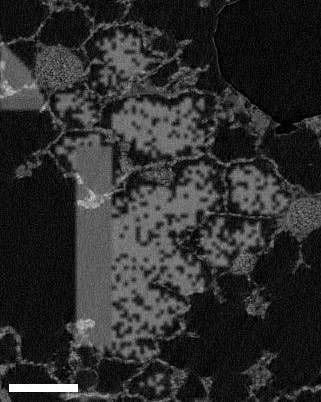
\includegraphics[height=\imsize]{img/Acini/2009f/mrg/R108C60Dt-mrg/acinus32/voxelsize1.48-every6slice/R108C60Dt-mrg-acinus32_45.png}% jpg is unedited!
		\label{subfig:60d_acinus32}%
	}%
	\hfill%
	%\subfloat[Animal 3, Acinus 38, Slice 29]{%
	\subfloat[Sample acinus from animal 3, Slice 29]{%
		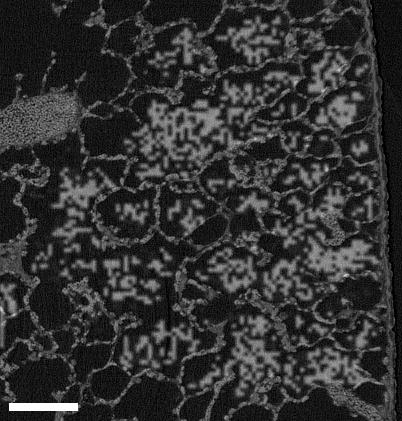
\includegraphics[height=\imsize]{img/Acini/2009f/mrg/R108C60Et-mrg/acinus38/voxelsize1.48-every6slice/R108C60Et-mrg-acinus38_29.png}% jpg is unedited!
		\label{subfig:60e_acinus38}%		
	}%
	\hfill%
	\caption{Typical sections of two acini showing large differences between the volumes estimated using MeVisLab and the STEPanizer.
		The inaccurate segmentation represents the reason why the MeVisLab volume was significantly smaller for these two acini than the volume estimated using the STEPanizer.
		Panel \protect\subref{subfig:60d_acinus32} shows minor segmentation errors due to noise observed in the airspace (dark spots inside grey region).
		Panel \protect\subref{subfig:60e_acinus38} shows large segmentation errors.
		Such large errors may arise due to brightness changes and noise in the dataset which render the threshold chosen unusable for some slices of the dataset.
		Scale bar: \SI{100}{\micro\meter}.}
	\label{fig:MeVisSegmentation}
\end{figure}

\section{Conclusions}
The hereby presented segmentation method is well suited to semi-automatically isolate individual acini from three-dimensional datasets for further stereological analysis.
To our best knowledge, the presented \replaced[id=st]{sequence of operations}{work flow} is the only one published to permit an easy, fast and semiautomatic extraction of individual acini.
After the extraction of the acini, a fully automated calculation of the volume of individual acini is possible, thus for the first time enabling the study of large amounts of individual acini in relatively short time.
This opens up the possibility to efficiently estimate biological parameters like volume and surface of individual acini, number of acini in the mammalian lung using well established stereological methods.

We know that we can correlate data obtained from synchrotron radiation based tomographic microscopy datasets to electron microscopy images, as shown before~\citep{Haberthuer2009}.
In this manuscript we show that it is also possible to extract meaningful biological parameters from samples imaged using ultrahigh resolution tomography without destroying the spatial information in the lung structure, \ie to perform a non-destructive analysis, something which is not possible with classic light microscopy imaging.

In the presented study, the segmentation of the individual acini was used to label the acinar structure on the virtual sections for stereological analysis, thus the segmentation and extraction of the individual acini is the prerequisite for the recognition of the acini.
This segmentation and extraction process represents the main amount of time spent evaluating the data, the calculation of the volume of the extracted acini can automatically be performed in a very short time.
With a more advanced segmentation algorithm it would be possible to automatically and accurately estimate the volume of a very large amount of acini in a very short time, since our proposed method for estimating the volumes of isolated individual acini is by magnitudes faster than manual stereological counting.

In addition, our proposed method may also be used to estimate changes in the lung structure (\eg acinar volume, number of alveoli, etc.) during the development of the lung.
We have only shown data for one time point in the lung development, but a stereological estimation of the presented parameters would also be possible for multiple time points during lung development or in different disease models like fibrosis or emphysem\added[id=st]{at}ic lungs.

\section{Acknowledgments}
We thank Federica Marone, Christoph Hintermüller and Bernd Pinzer for their committed support at the TOMCAT beamline.
Milo Hindennach from Fraunhofer MEVIS provided the \href{http://www.mevis-research.de/cgi-bin/discus/board-auth.cgi?lm=1282233250&file=/839/11760.html}{Manhole cover module in MeVisLab}.
We thank Mohammed Ouanella for expert technical assistance and embedding of the samples.

\section{Grants}
This work has been supported by the grants 3100A0-109874 and 310030-125397 of the Swiss National Science Foundation.

\section*{Contributions}
\begin{itemize}
	\item David Haberthür performed data acquisition, estimated acinar volumes and surfaces, designed and performed analysis of data and wrote the manuscript.
	\item Sébastien F. Barré performed data acquisition and contributed to analysis of data.
	\item Stefan A. Tschanz obtained the samples and contributed to stereological analysis.
	\item Evelyne Yao prepared the samples and estimated alveolar numbers of the acini.
	\item Marco Stampanoni designed the beamline and contributed to writing.
	\item Johannes C. Schittny conceived and designed the study, obtained the samples, performed the data acquisition and contributed to writing.
\end{itemize}

\section{Disclosures}
No \href{http://www.the-aps.org/mm/Publications/Preparing-Your-Manuscript#conflicts}{conflicts of interest} exist for any author of this manuscript.

\ifJCS
	\singlespacing
\else
\fi

\bibliographystyle{plainnat}
\bibliography{../library}

\end{document}